\documentclass{beamer}
\usetheme{default}
\usepackage{tikz}
\usetikzlibrary{arrows,shapes.arrows,positioning,shapes}
\usepackage{graphicx}
\usepackage{hyperref}
\usepackage{comment}
\usepackage{tikz}
\beamertemplatenavigationsymbolsempty
\usetikzlibrary{arrows,shapes.arrows,positioning,shapes}
\newcommand\red[1]{{\color{red}#1}}
\newcommand\bred[1]{{\color{red}\textbf{#1}}}
\newcommand\blue[1]{{\color{blue}#1}}
\newcommand\bblue[1]{{\color{blue}\textbf{#1}}}
\newcommand\green[1]{{\color{olive}#1}}
\newcommand\bgreen[1]{{\color{olive}\textbf{#1}}}
\newcommand\black[1]{{\color{black}#1}}
\newcommand\white[1]{{\color{white}#1}}
\newcommand\E{\text{E}}
\newcommand\V{\text{V}}
\renewcommand\P{\text{P}}

\title{Participating in the Fragile Families Challenge Activity}

\author{{\small Matthew Salganik, Ian Lundberg, Alex Kindel, Sara McLanahan,\\and people from around the world}}

%\institute[]
%{
%  Department of Sociology, Office of Population Research, \& \\Center for Research on Child Wellbeing, Princeton University}

\date{Summer Institutes in Computational Social Science\\June 21, 2019 \\ \vfill
\begin{flushleft}{\scriptsize
Fragile Families Challenge is supported by the Russell Sage Foundation. Board of Advisors: Jeanne Brooks-Gunn, Kathryn Edin, Barbara Engelhardt, Irwin Garfinkel, Moritz Hardt, Dean Knox, Nicholas Lemann, Karen Levy, Sara McLanahan, Arvind Narayanan, Timothy Nelson, Matthew Salganik, Brandon Stewart \& Duncan Watts.} 
\includegraphics[width=0.05\textwidth]{figures/cc-by.png}
\end{flushleft}
}

%\pgfdeclareimage[height=1cm]{university-logo}{ff_logo.jpg}
%\logo{\pgfuseimage{university-logo}}

%%%%%%%%%%%%%%%%%%%%%%%%%%%%%%
\begin{document}

\begin{frame}
  \titlepage
\end{frame}

%%%%%%%%%%%%%%%%%%%%%%%%%%%
\begin{frame}

\begin{center}
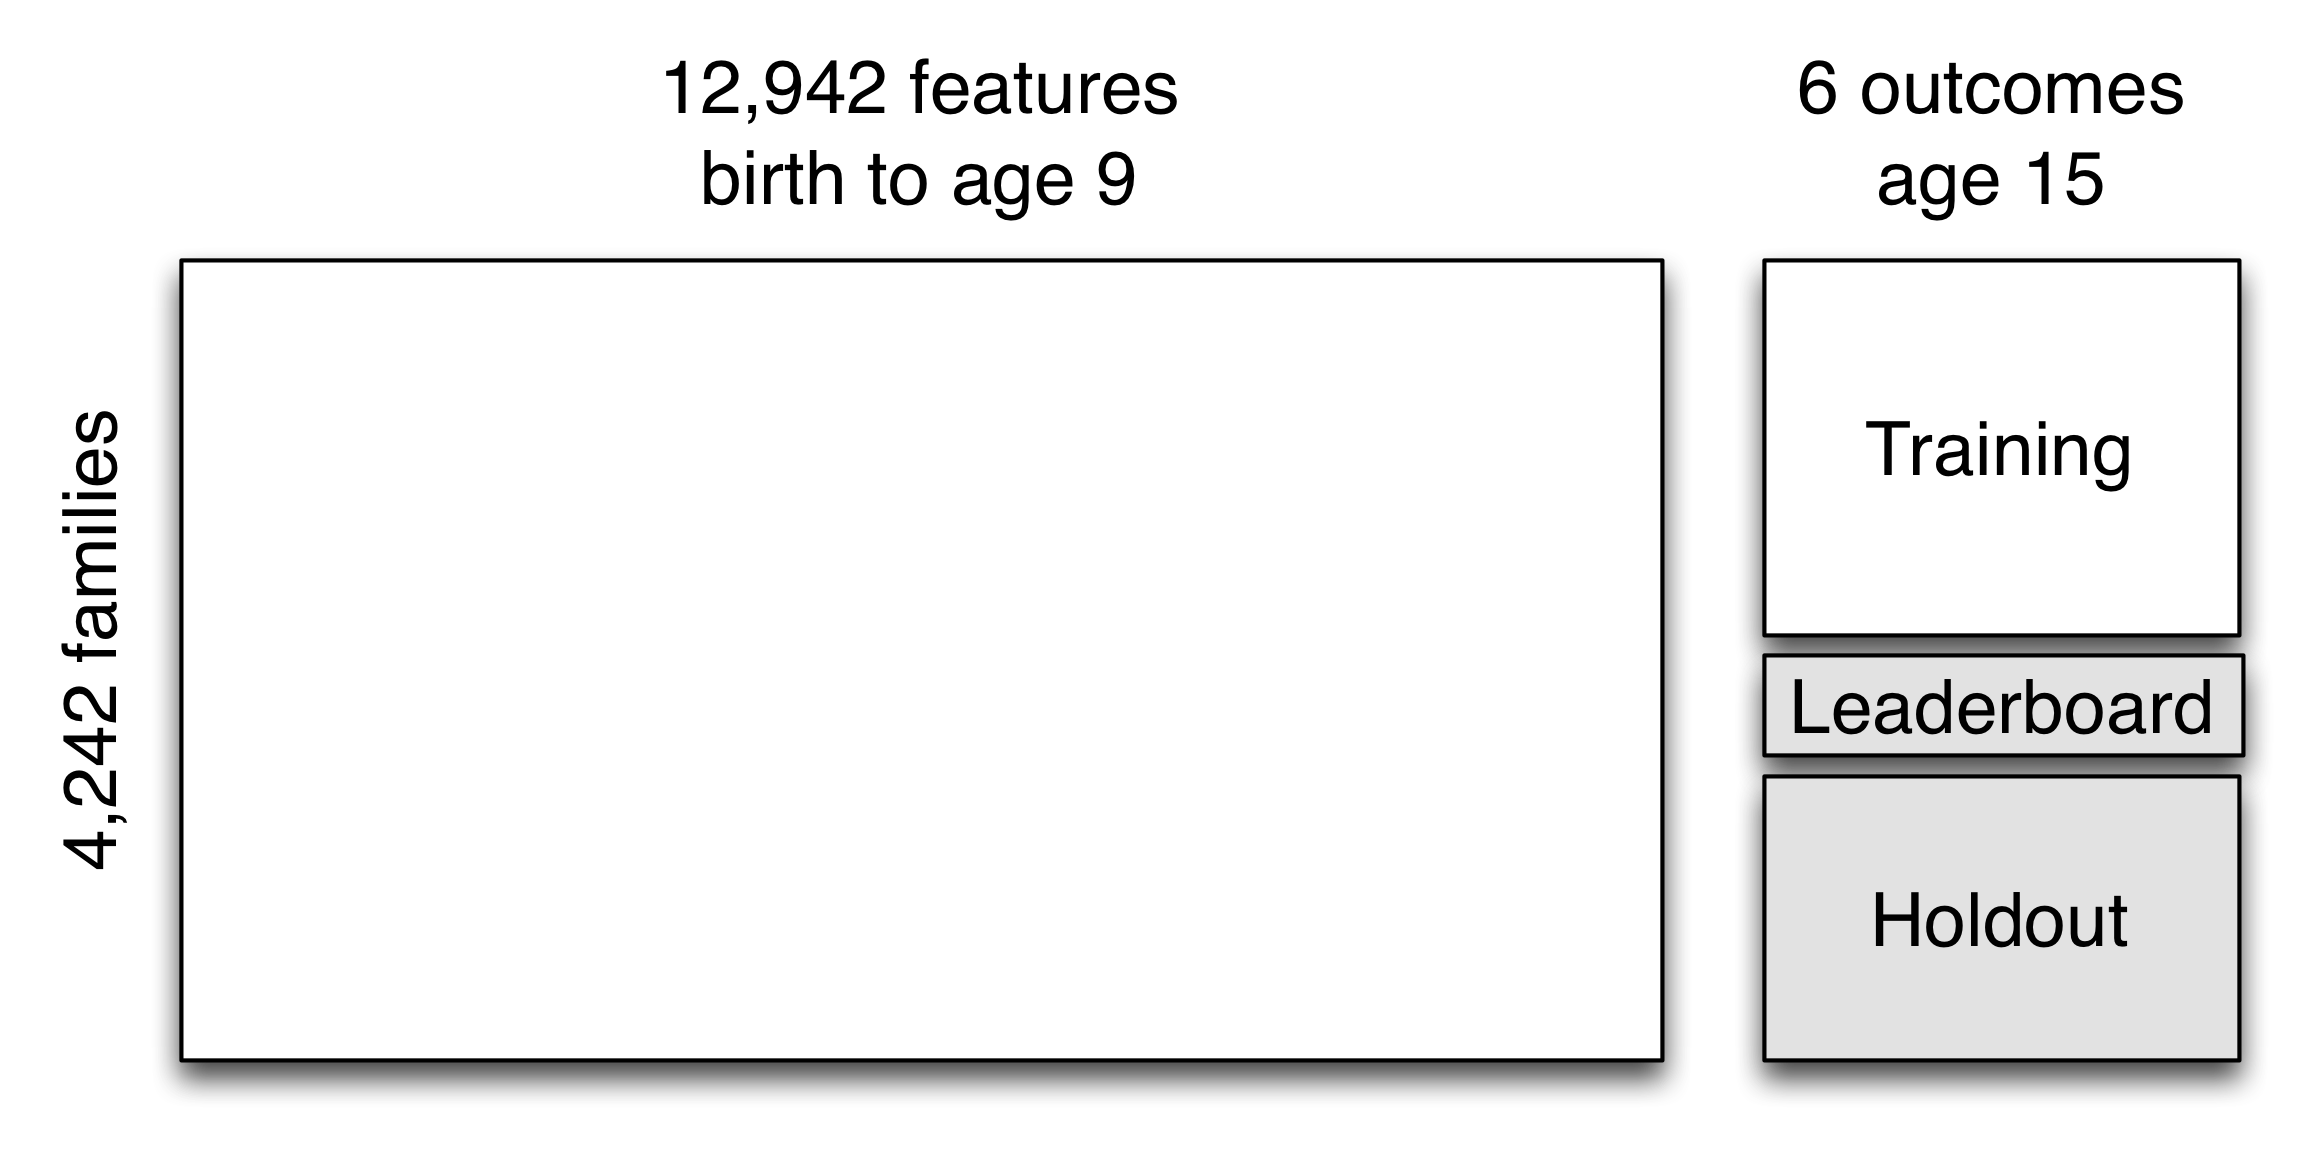
\includegraphics[width=\textwidth]{figures/ffc_design_matrix_ml}
\end{center}

\end{frame}
%%%%%%%%%%%%%%%%%%%%%%%%%
\begin{frame}

\Large{
\begin{center}
Introducing the outcome variables
\end{center}
}

\end{frame}
%%%%%%%%%%%%%%%%%%%%%%%%%
\begin{frame}

\Large{
\begin{center}
GPA\footnote{Learn more at \url{http://www.fragilefamilieschallenge.org/gpa/} \vskip .2cm}
\pause \vskip .5cm
How do kids beat the odds academically?
\end{center}
}

\end{frame}
%%%%%%%%%%%%%%%%%%%%%%%%%
\begin{frame}{GPA\footnote{This variable is reverse-coded in the data file so that higher values represent higher GPAs.}}

\centering
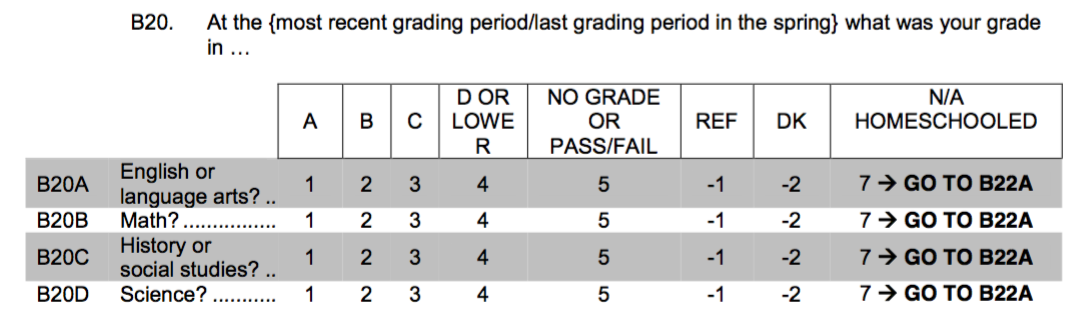
\includegraphics[width = .9\textwidth]{figures/GPA_questionnaire}

\end{frame}
%%%%%%%%%%%%%%%%%%%%%%%%%
\begin{frame}

\centering
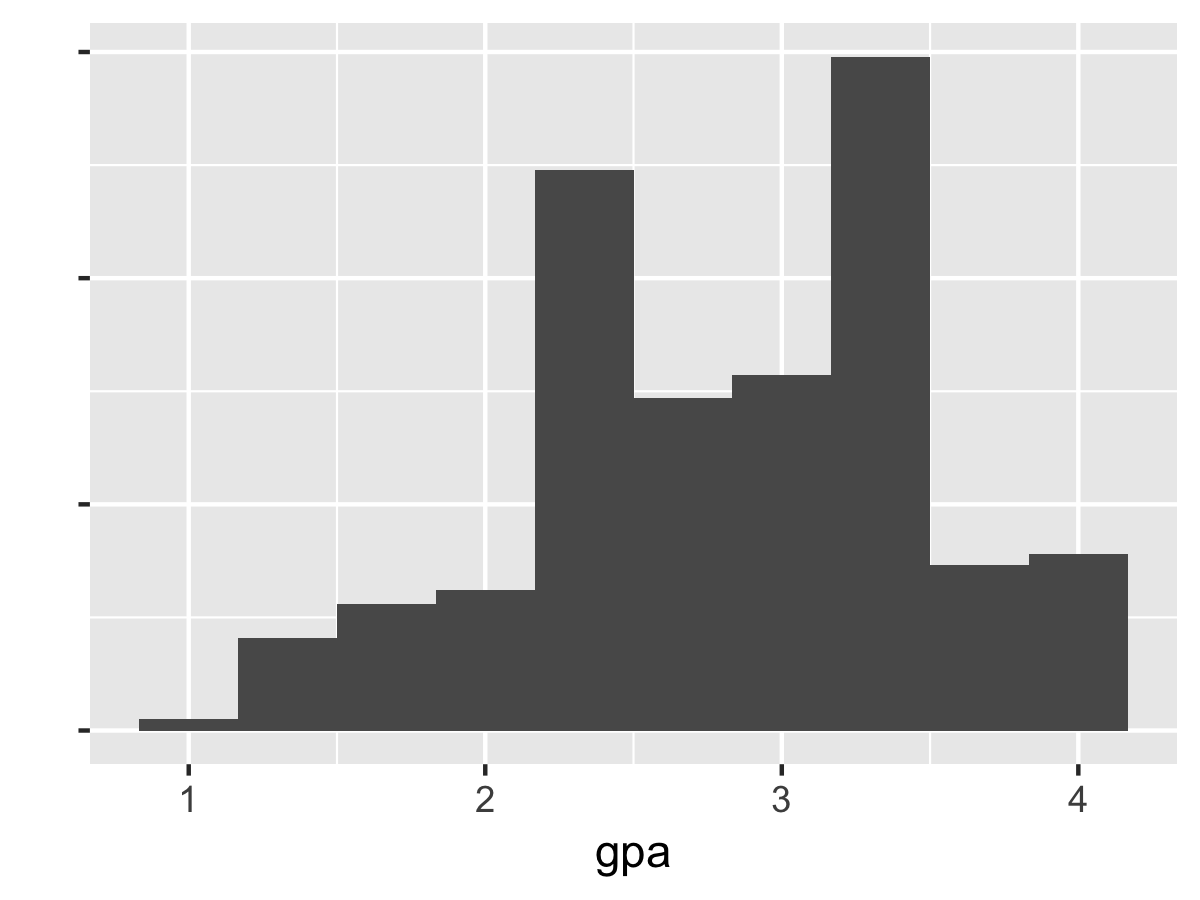
\includegraphics[width = .9\textwidth]{figures/gpaDist}

\end{frame}
%%%%%%%%%%%%%%%%%%%%%%%%%
\begin{frame}
\begin{center}
\Large{
``Grit'' predicts success, possibly more than IQ.\footnote{Learn more at \url{http://www.fragilefamilieschallenge.org/grit/}\vskip .2cm} \vskip .3cm

\includegraphics[width = .3\textwidth]{figures/duckworth_grit_2016_cover} \vskip .3cm \pause
What makes some kids gritty?
} 
\end{center}
\end{frame}
%%%%%%%%%%%%%%%%%%%%%%%%%%%
\begin{frame}{Grit\footnote{This variable is reverse-coded in the data file so that higher values represent more grit.}}

\centering
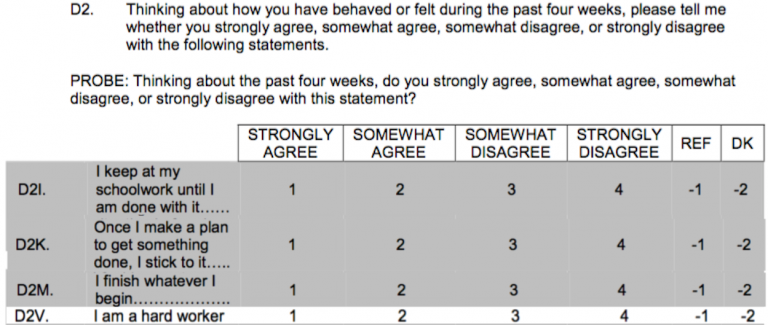
\includegraphics[width = .9\textwidth]{figures/grit_questionnaire2}

\end{frame}
%%%%%%%%%%%%%%%%%%%%%%%%%
\begin{frame}

\centering
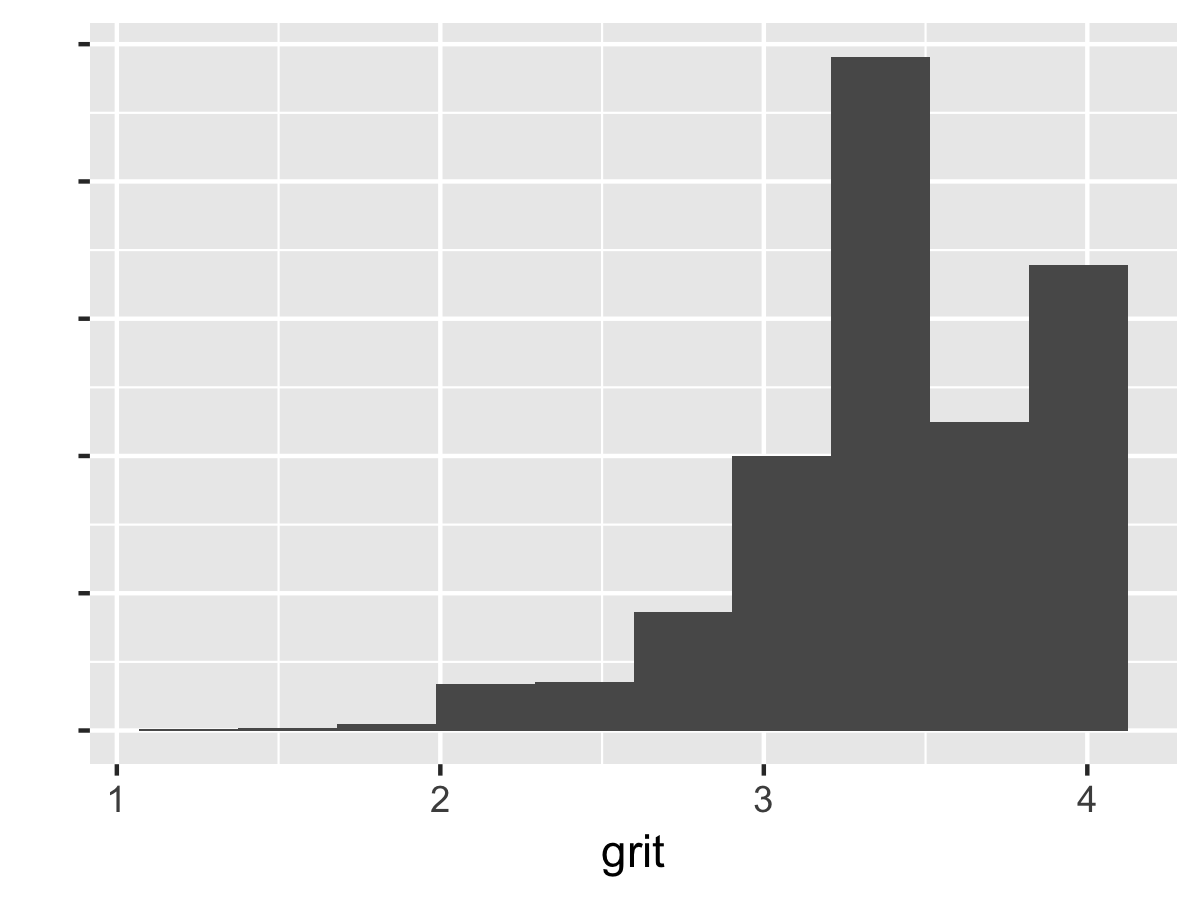
\includegraphics[width = .9\textwidth]{figures/gritDist}

\end{frame}
%%%%%%%%%%%%%%%%%%%%%%%%%
\begin{frame}

\Large{
\begin{center}
Material hardship\footnote{Learn more at \url{http://www.fragilefamilieschallenge.org/material-hardship/}\vskip .2cm} \pause \vskip .3cm 
What unmeasured predictors are associated with families unexpectedly escaping severe deprivation? 
\pause \vskip .3cm What sends families unexpectedly into deep poverty?
\end{center}
}

\end{frame}
%%%%%%%%%%%%%%%%%%%%%%%%%%%
\begin{frame}{Material hardship}

\centering
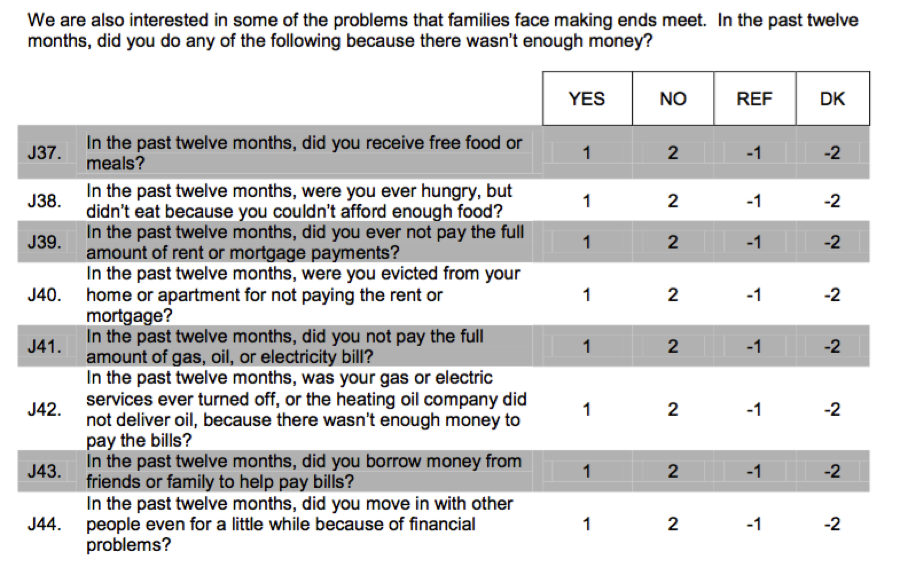
\includegraphics[width = .9\textwidth]{figures/materialHardship_questionnaireA}

\end{frame}
%%%%%%%%%%%%%%%%%%%%%%%%%%%
\begin{frame}{Material hardship}

\centering
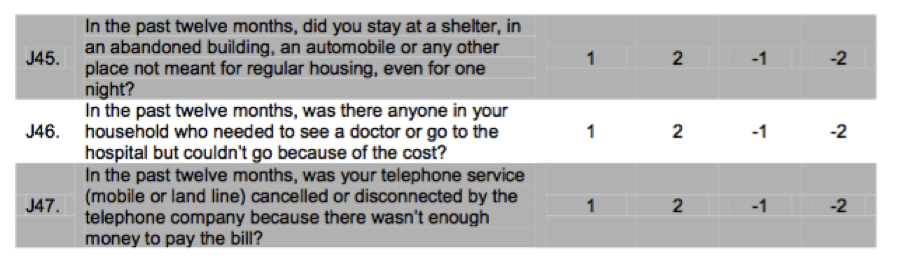
\includegraphics[width = .9\textwidth]{figures/materialHardship_questionnaireB}

\end{frame}
%%%%%%%%%%%%%%%%%%%%%%%%%
\begin{frame}

\centering
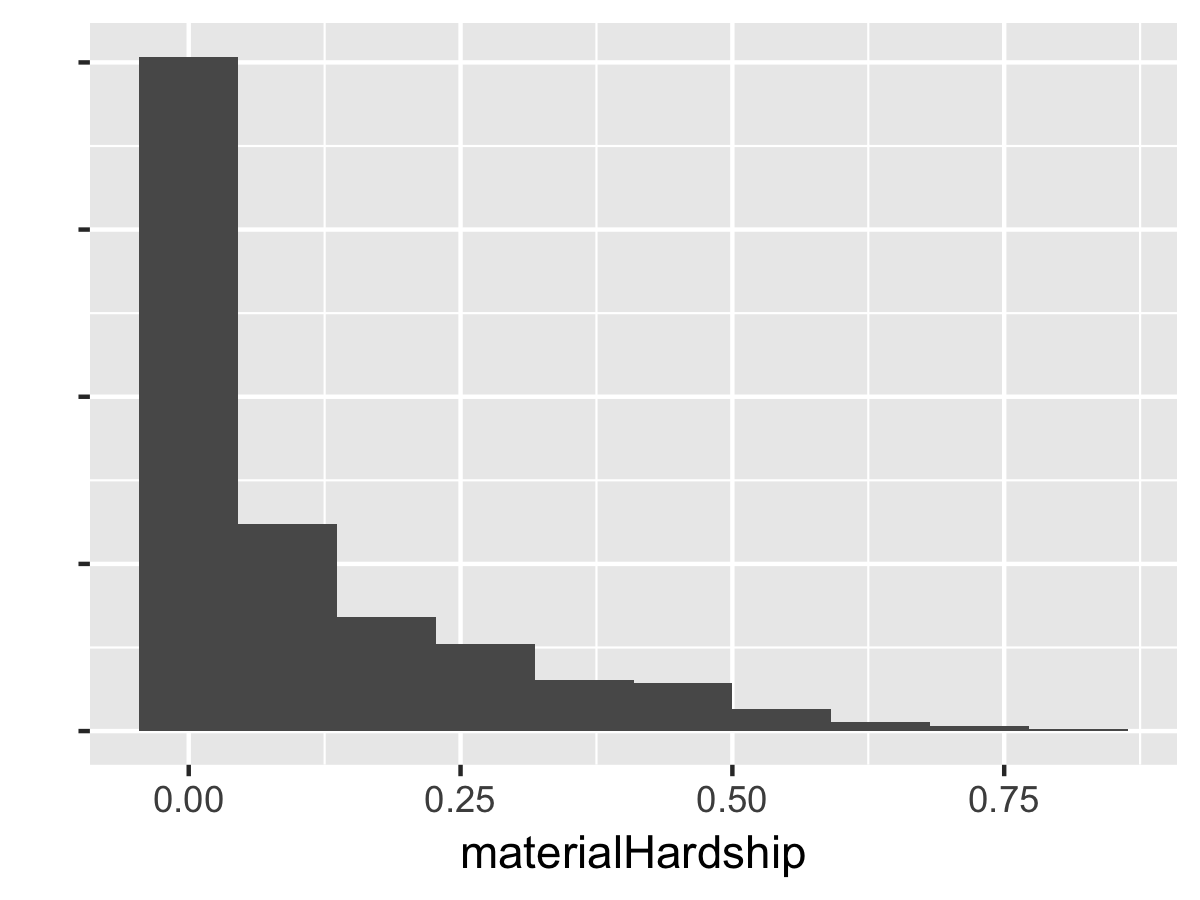
\includegraphics[width = .9\textwidth]{figures/materialHardshipDist}

\end{frame}
%%%%%%%%%%%%%%%%%%%%%%%%%
\begin{frame}

\Large{
\begin{center}
Eviction\footnote{Learn more at \url{http://www.fragilefamilieschallenge.org/eviction/}\vskip .2cm}
\pause \vskip .5cm
Does housing eviction \textbf{cause} worse outcomes as kids transition to adulthood?\footnote{Note: You will just create propensity scores for eviction given background variables; causal inference comes in the second stage of the Challenge when outcomes are measured several years from now.}
\end{center}
}

\end{frame}
%%%%%%%%%%%%%%%%%%%%%%%%%%%
\begin{frame}{Eviction}

\centering
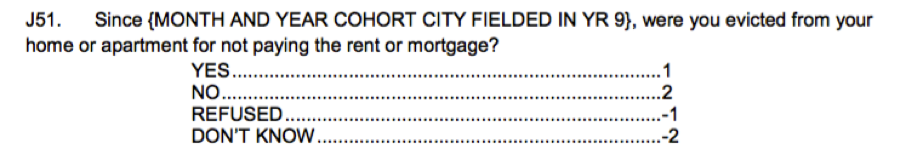
\includegraphics[width = .9\textwidth]{figures/eviction_questionnaire}

\end{frame}
%%%%%%%%%%%%%%%%%%%%%%%%%
\begin{frame}

\centering
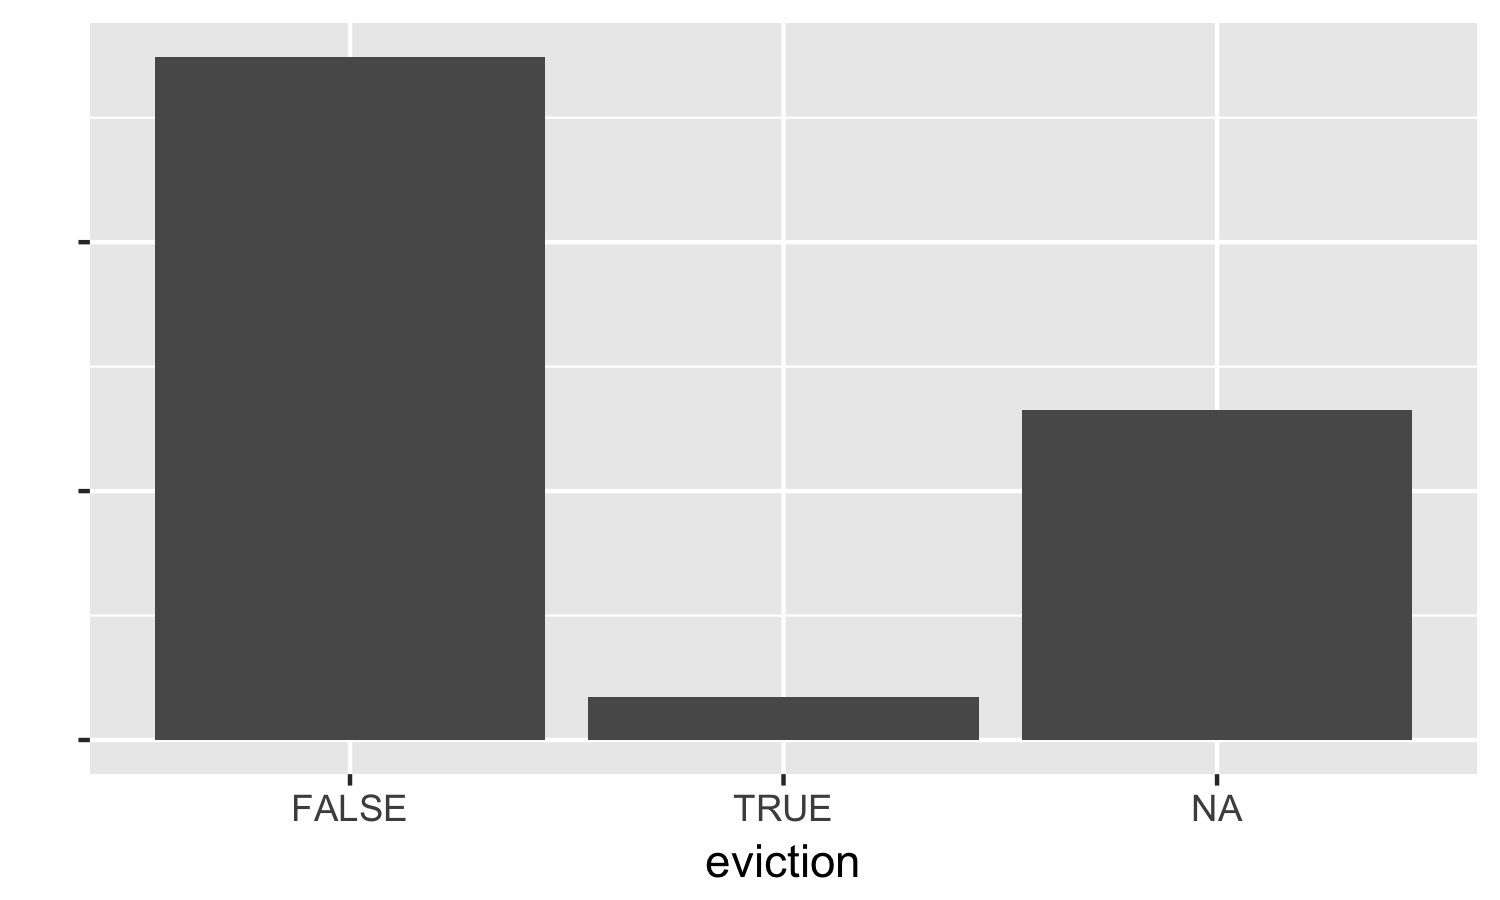
\includegraphics[width = .9\textwidth]{figures/evictionDist}

\end{frame}
%%%%%%%%%%%%%%%%%%%%%%%%%
\begin{frame}

\Large{
\begin{center}
Caregiver layoff\footnote{Learn more at \url{http://www.fragilefamilieschallenge.org/layoff/}\vskip .2cm}
\pause \vskip .5cm 
Does layoff of a caregiver \textbf{cause} collateral damage for kids?\footnote{Note: You will just create propensity scores for caregiver layoff given background variables; causal inference comes in the second stage of the Challenge when outcomes are measured several years from now.}
\end{center}
}

\end{frame}
%%%%%%%%%%%%%%%%%%%%%%%%%%%
\begin{frame}{Caregiver layoff}

\centering
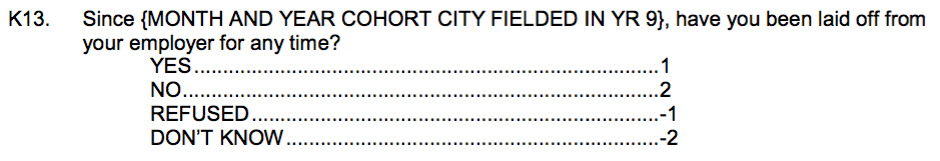
\includegraphics[width = .9\textwidth]{figures/layoff_questionnaire}

\end{frame}
%%%%%%%%%%%%%%%%%%%%%%%%%
\begin{frame}

\centering
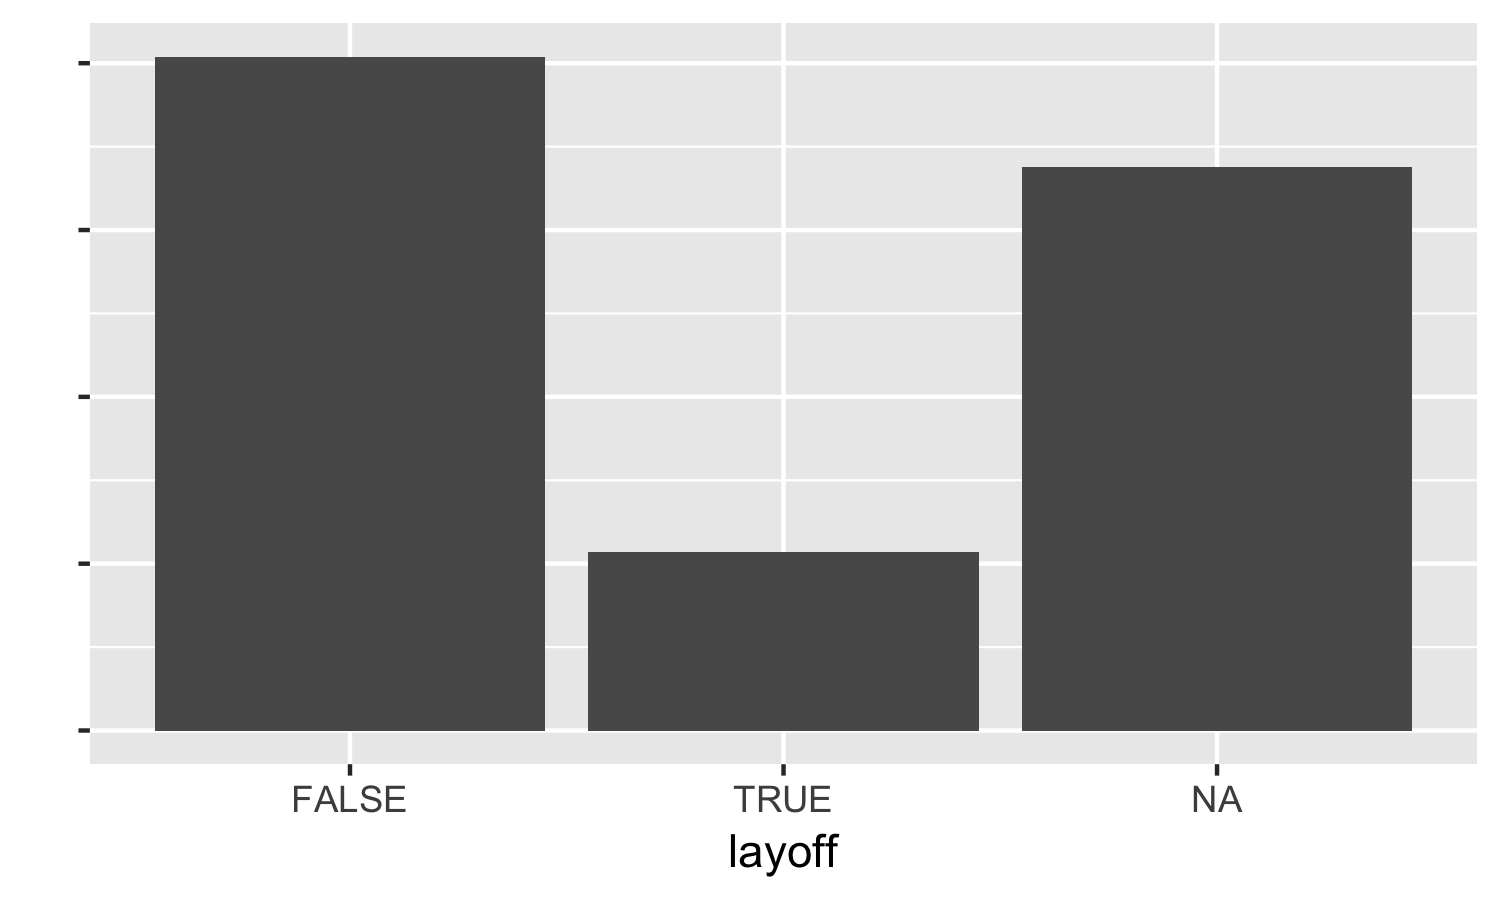
\includegraphics[width = .9\textwidth]{figures/layoffDist}

\end{frame}
%%%%%%%%%%%%%%%%%%%%%%%%%
\begin{frame}

\Large{
\begin{center}
Job training\footnote{Learn more at \url{http://www.fragilefamilieschallenge.org/job-training/}\vskip .2cm}
\pause \vskip .5cm 
Does job training for a caregiver \textbf{cause} collateral benefits for children?\footnote{Note: You will just create propensity scores for job training given background variables; causal inference comes in the second stage of the Challenge when outcomes are measured several years from now.}
\end{center}
}

\end{frame}
%%%%%%%%%%%%%%%%%%%%%%%%%%%
\begin{frame}{Caregiver job training}

\centering
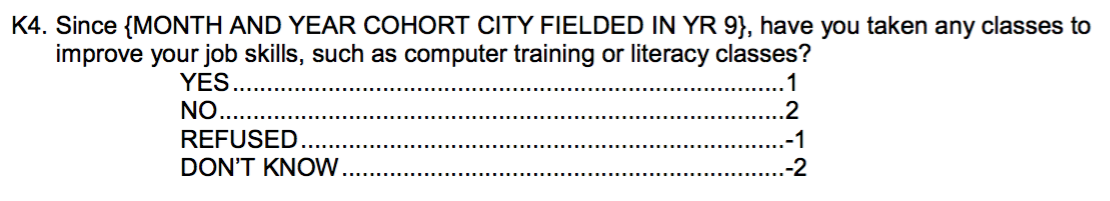
\includegraphics[width = .9\textwidth]{figures/jobTraining_questionnaire}

\end{frame}
%%%%%%%%%%%%%%%%%%%%%%%%%
\begin{frame}

\centering
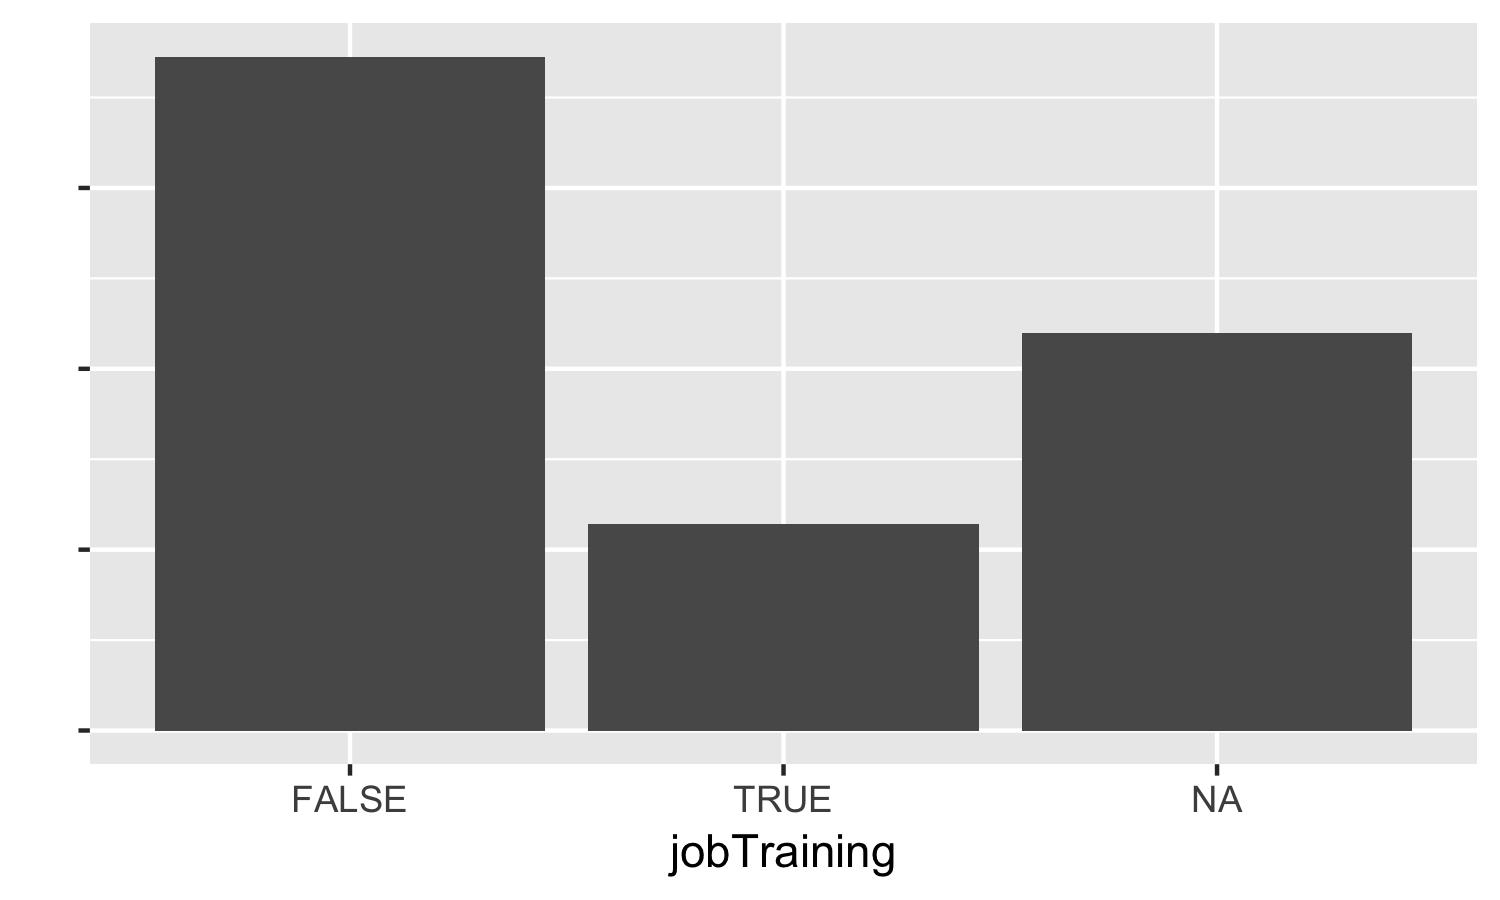
\includegraphics[width = .9\textwidth]{figures/jobTrainingDist}

\end{frame}
%%%%%%%%%%%%%%%%%%%%%%%%%%%
\begin{frame}

\Large{
\begin{center}
Introducing the data
\end{center}
}

\end{frame}
%%%%%%%%%%%%%%%%%%%%%%%%%
\begin{frame}

\textbf{The Fragile Families and Child Wellbeing Study is a dataset of real people who have selflessly opened up their lives to us for the last 15 years so that their experiences can contribute to scientific research. By participating in the Fragile Families Challenge, you become a collaborator in this project. It is of the utmost importance that you respect the families in the data by using what they have told us responsibly.}

\end{frame}
%%%%%%%%%%%%%%%%%%%%%%%%%
\begin{frame}

\begin{itemize}
\item Before you have access to the data, you will sign a data use agreement
\pause
\item After this activity you will delete the data from your computer
\pause
\item If you want to keep working with the data afterwards, you can apply for access through the Fragile Families website
\end{itemize}

\end{frame}
%%%%%%%%%%%%%%%%%%%%%%%%
\begin{frame}

\begin{center}
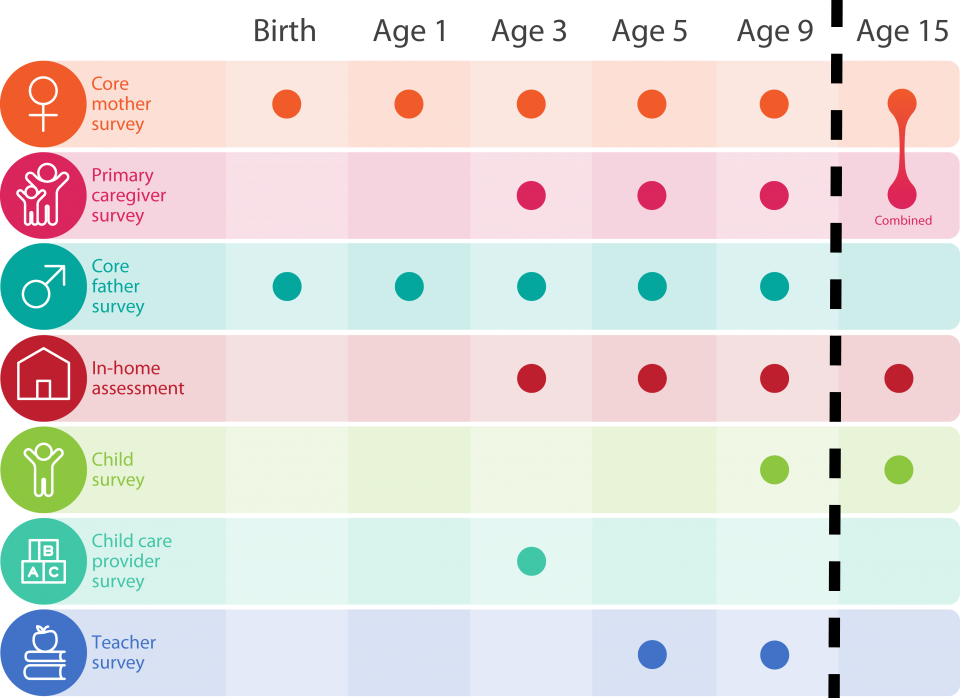
\includegraphics[width=\textwidth]{figures/ff_design_public2}
\end{center}

\end{frame}
%%%%%%%%%%%%%%%%%%%%%%%%%
\begin{frame}

\begin{center}
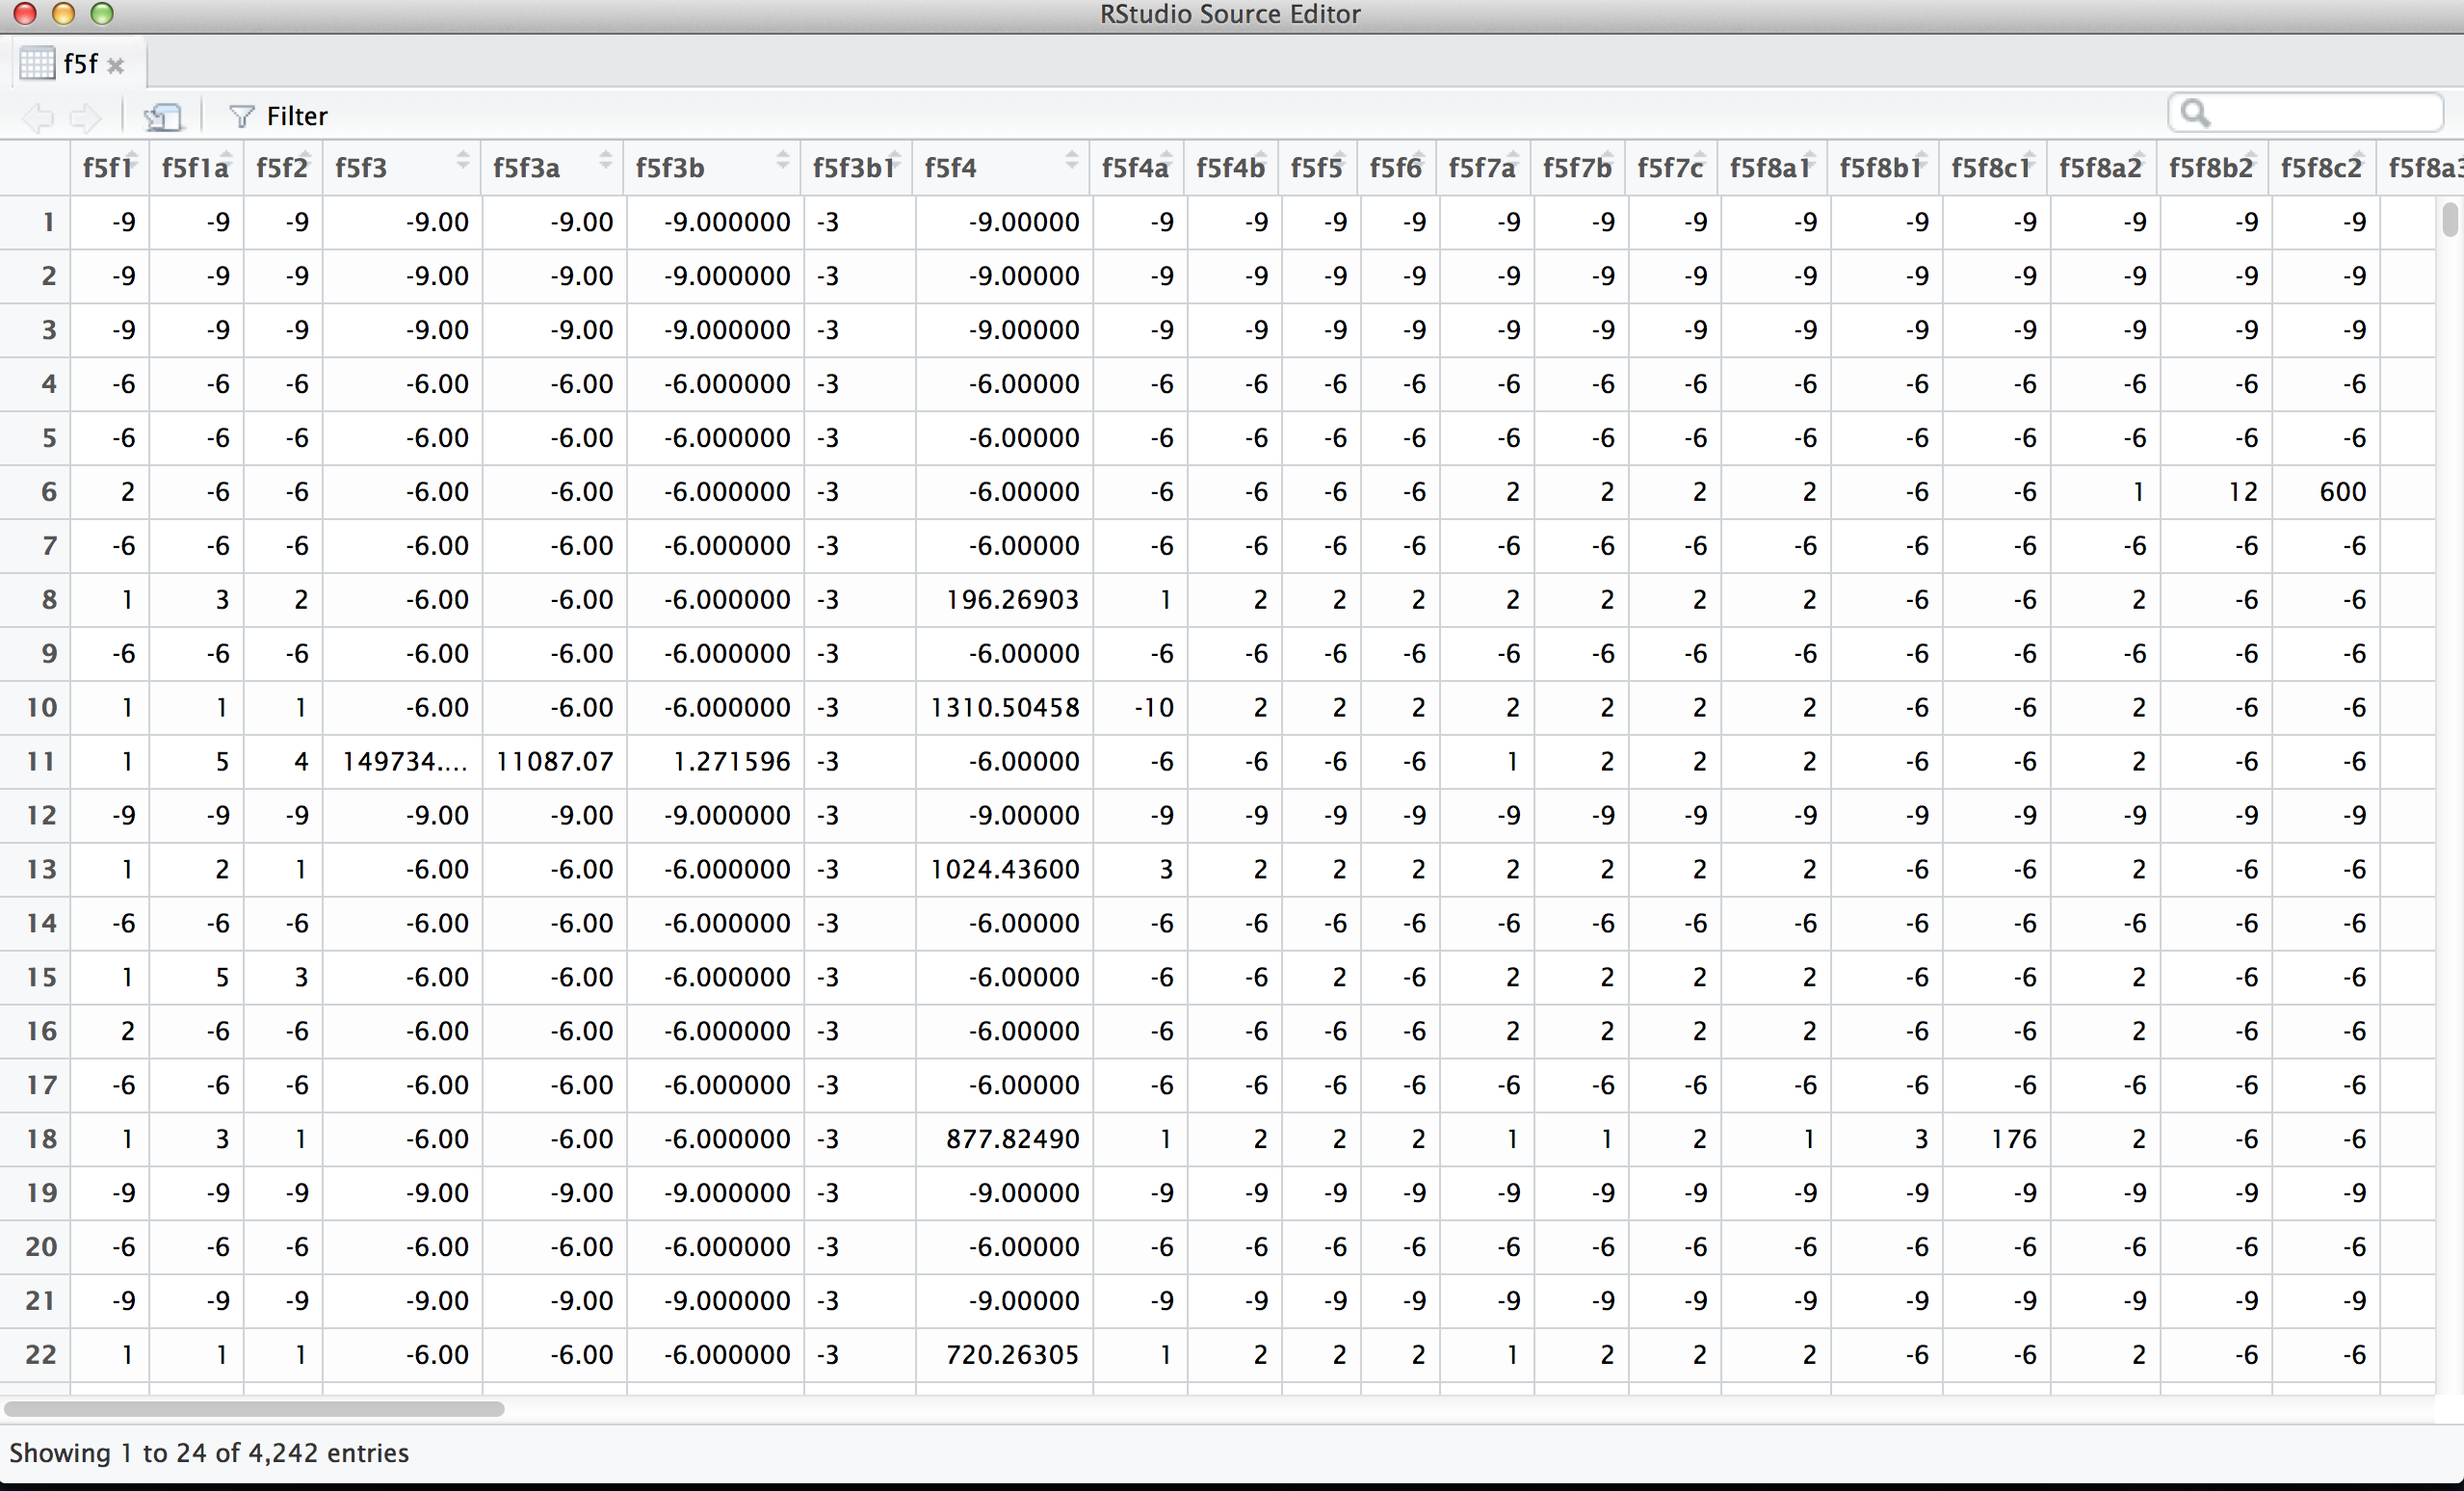
\includegraphics[width=\textwidth]{figures/ffc_rawdata_f5f}
\end{center}

\end{frame}
%%%%%%%%%%%%%%%%%%%%%%%%%
\begin{frame}

\begin{center}
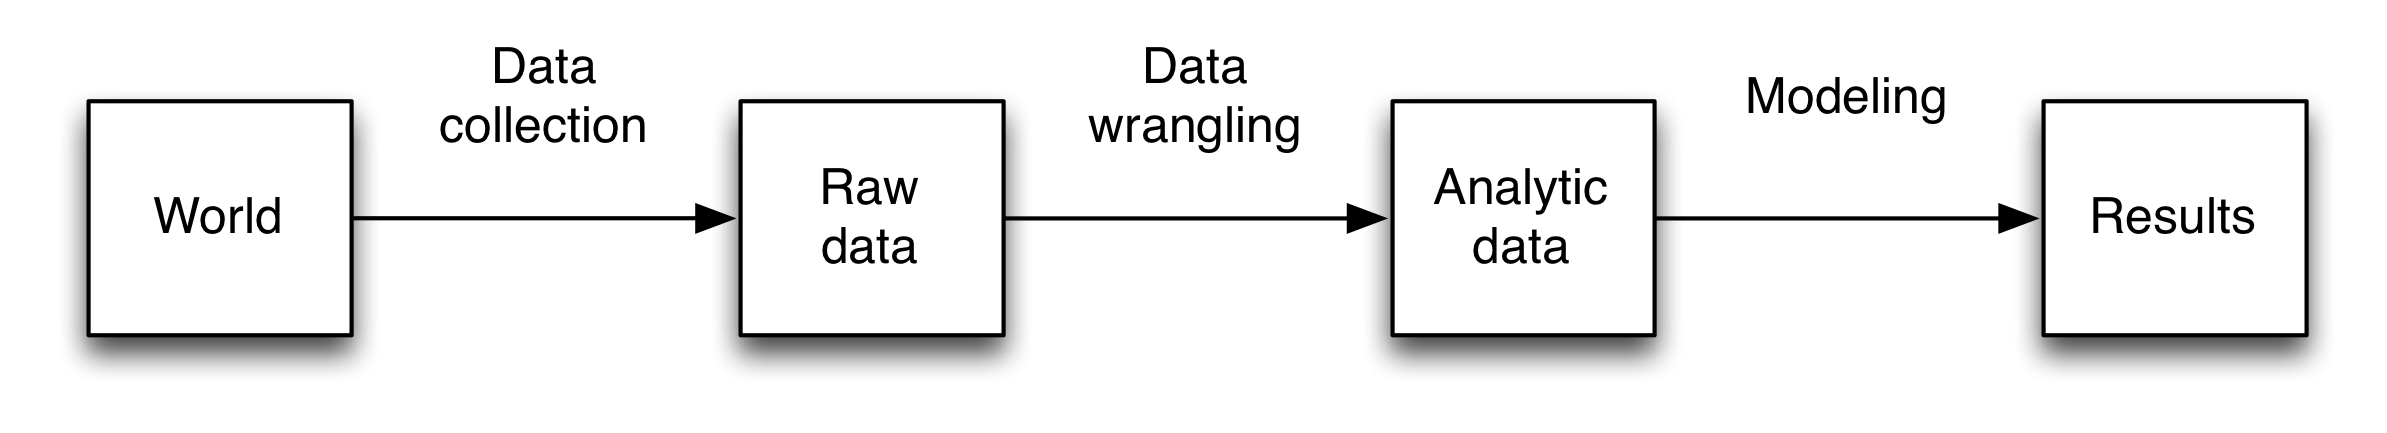
\includegraphics[width=\textwidth]{figures/scientific_pipeline}
\end{center}

\end{frame}
%%%%%%%%%%%%%%%%%%%%%%%%%
\begin{frame}

\begin{itemize}
\item A team of people\footnote{Alexander Kindel, Vineet Bansal, Kristin Catena, Thomas Hartshorne, Kate Jaeger, Dawn Koffman, Sara McLanahan, Maya Phillips, Shiva Rouhani, Ryan Vinh, Matthew Salganik.} has spent months making the data easier to use. \pause
\item Is it possible to do better than last time? Or, is there a fundamental limit with this data and this task? \pause
\item Let's see if it improves performance, \pause and let's see if you can help make this easier for future researchers.
\end{itemize}

\end{frame}
%%%%%%%%%%%%%%%%%%%%%%%%%
\begin{frame}

How do I know what these variables are? 

\begin{center}
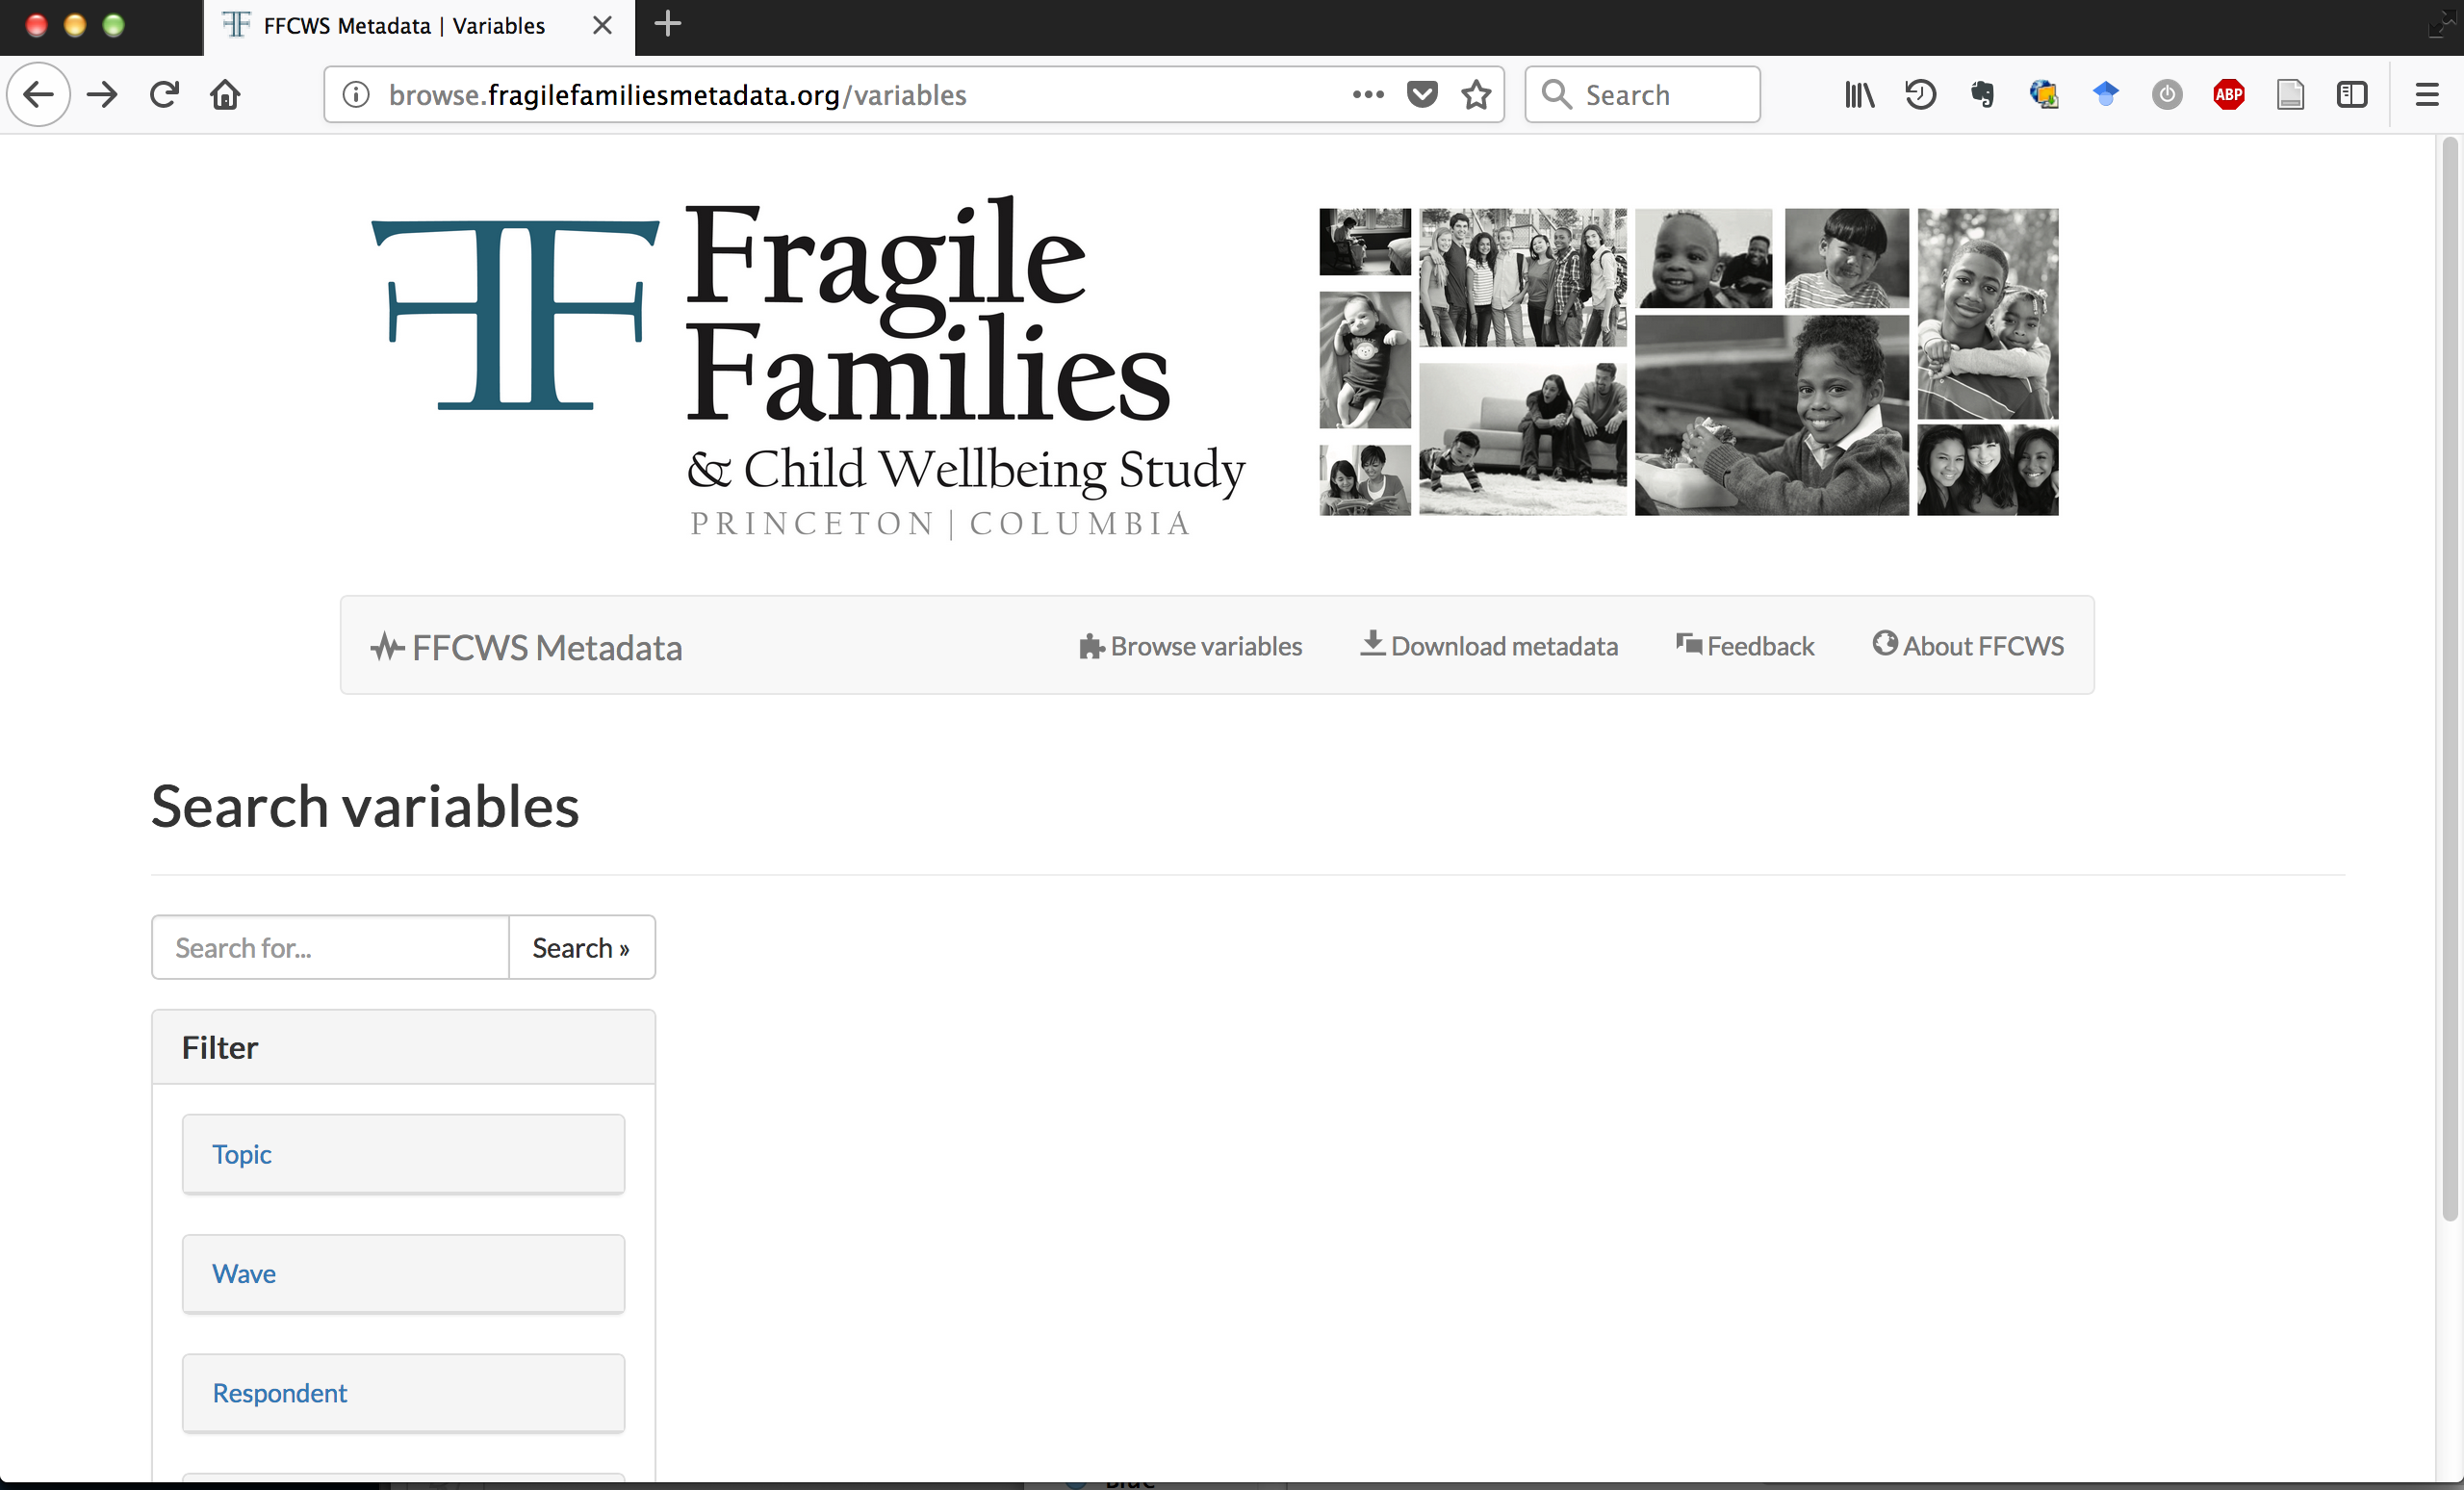
\includegraphics[width=\textwidth]{figures/ff_metadata_browser}
\end{center}

\vfill

\url{http://metadata.fragilefamilies.princeton.edu/variables}

\end{frame}
%%%%%%%%%%%%%%%%%%%%%%%%%%%
\begin{frame}

Introducing \texttt{cm1relf}\\

\url{metadata.fragilefamilies.princeton.edu/variables/cm1relf}

\end{frame}
%%%%%%%%%%%%%%%%%%%%%%%%%%%
\begin{frame}

You can filter variables by:
\begin{itemize}
\item Topic
\item Wave
\item Respondent
\item Variable Type (e.g., continuous, ordered categorical, unordered categorical, etc).
\end{itemize}

\end{frame}	
%%%%%%%%%%%%%%%%%%%%%%%%%%%
\begin{frame}

Why \texttt{cm1relf}? \pause

\begin{center}
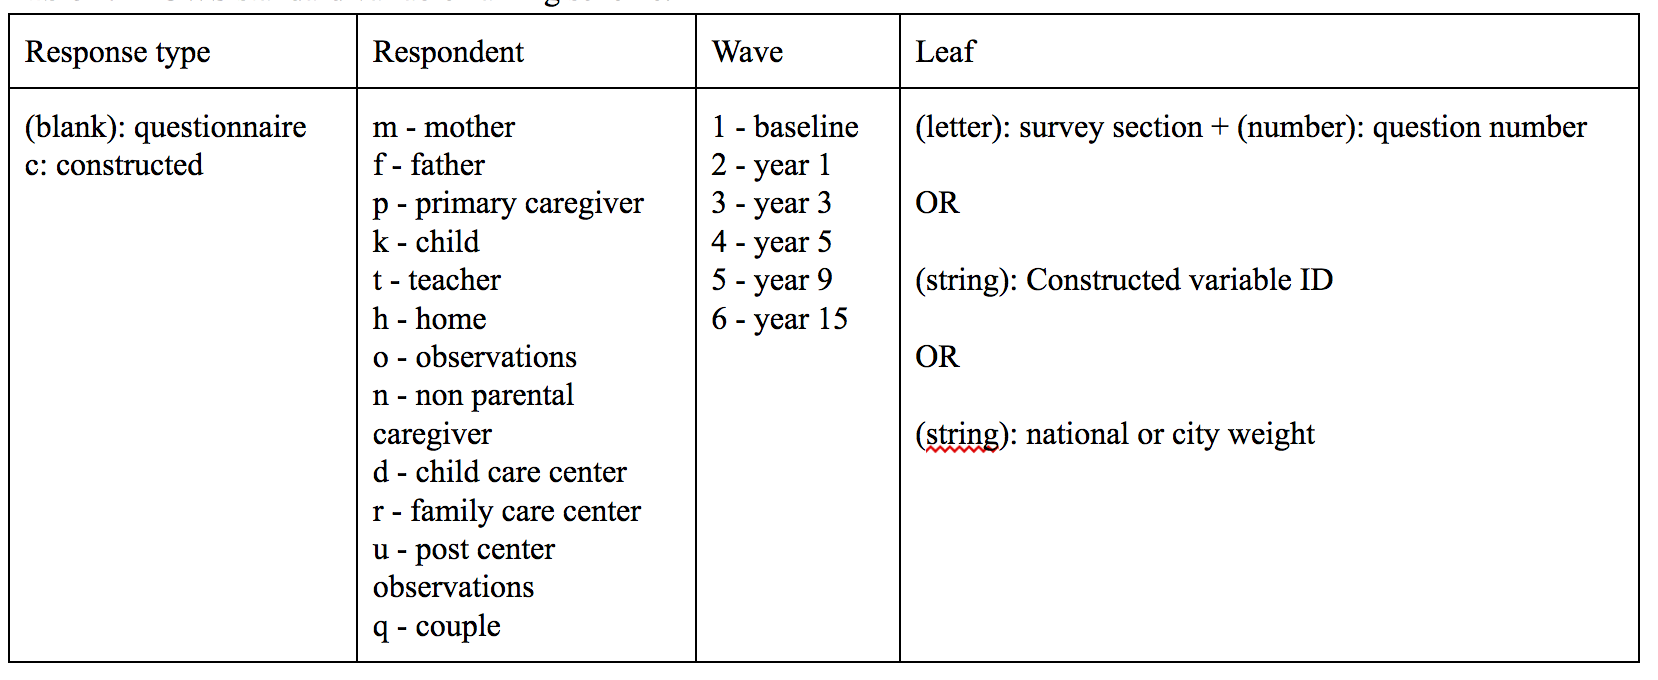
\includegraphics[width=\textwidth]{figures/ff_variablename_standards}
\end{center}

\end{frame}
%%%%%%%%%%%%%%%%%%%%%%%%%%
\begin{frame}

Want direct access to the metadata?  \pause No problem

\begin{itemize}
\item API: \url{api.metadata.fragilefamilies.princeton.edu}
\item Python package: \url{github.com/fragilefamilieschallenge/ffmetadata-py}
\item R package: \url{github.com/fragilefamilieschallenge/ffmetadata}
\item Raw metadata: \url{api.fragilefamiliesmetadata.org/get_metadata}
\end{itemize}

\end{frame}
%%%%%%%%%%%%%%%%%%%%%%%%%%%
\begin{frame}

\centering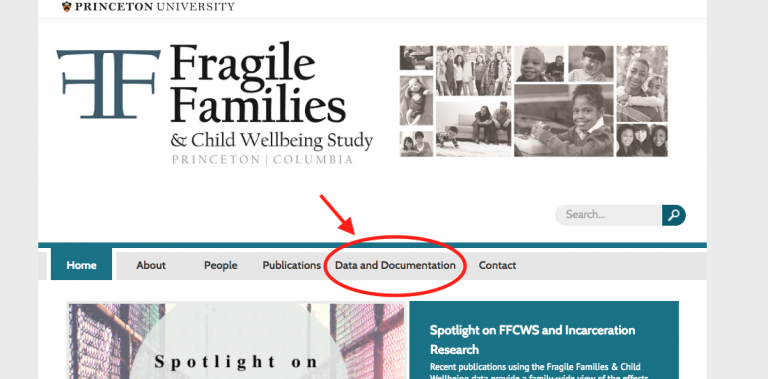
\includegraphics[width = .8\textwidth]{figures/Doc1}

\end{frame}
%%%%%%%%%%%%%%%%%%%%%%%%%%%
\begin{frame}

\centering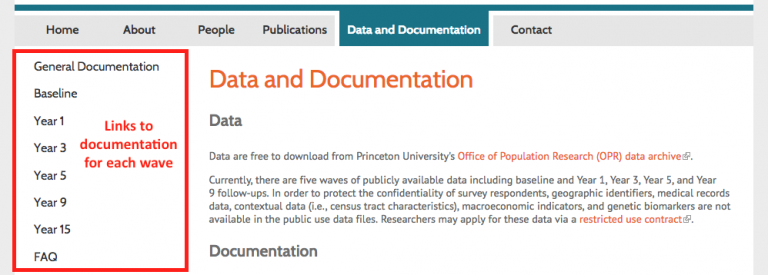
\includegraphics[width = .8\textwidth]{figures/Doc2}

\end{frame}
%%%%%%%%%%%%%%%%%%%%%%%%%%%
\begin{frame}

\centering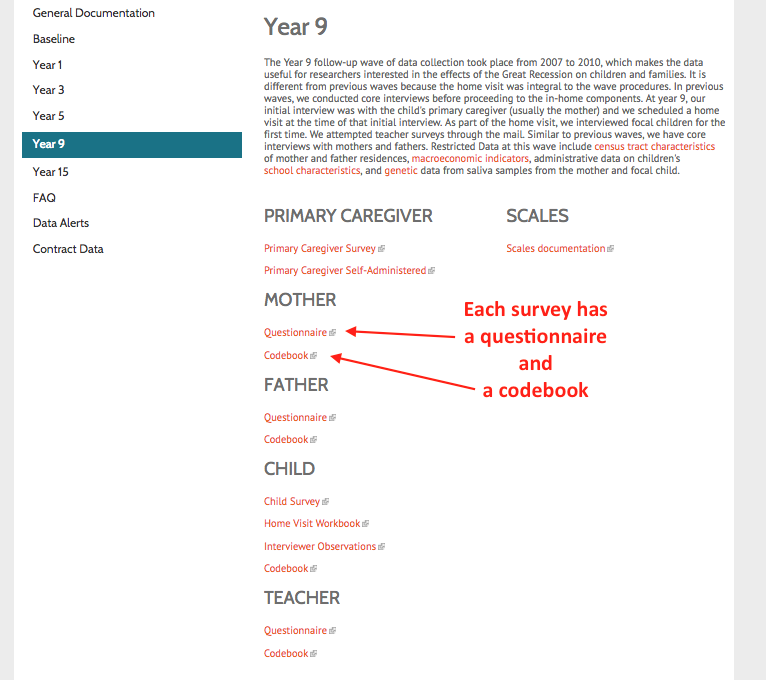
\includegraphics[width = .8\textwidth]{figures/Doc3}

\end{frame}
%%%%%%%%%%%%%%%%%%%%%%%%%%%
\begin{frame}

Questionnaire:\\
\centering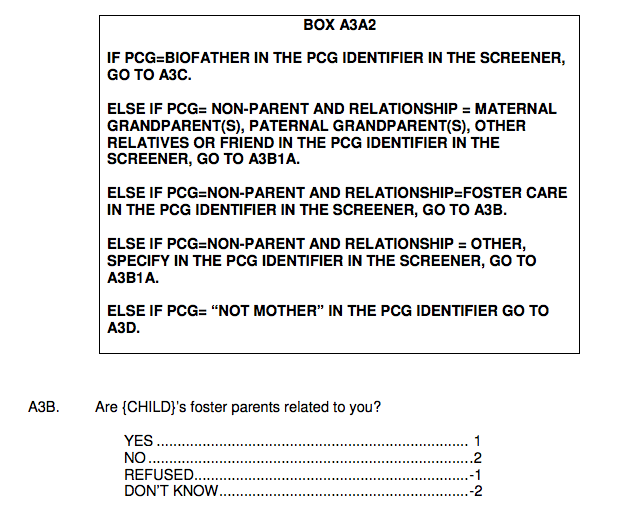
\includegraphics[width = .8\textwidth]{figures/Doc4}

\end{frame}
%%%%%%%%%%%%%%%%%%%%%%%%%%%
\begin{comment}
\begin{frame}

In the corresponding codebook, we see the count of respondents who gave each answer:
\vskip .3cm
\begin{center}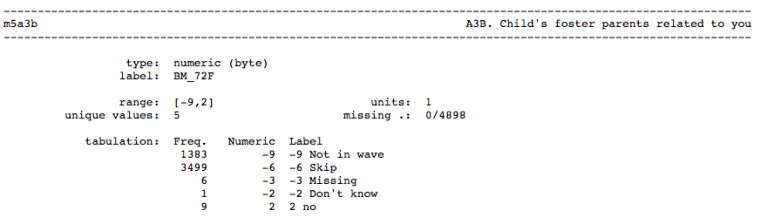
\includegraphics[width = .8\textwidth]{figures/Doc5}\end{center}
\vskip .3cm \pause
Things to note here:
\vskip .3cm \pause
\begin{itemize}
\item The question referred to in the questionnaire as A3B is called m5a3b in the codebook. \pause
\item There are missing codes.
\end{itemize}

\end{frame}
\end{comment}
%%%%%%%%%%%%%%%%%%%%%%%%%%%
\begin{frame}

\begin{center}
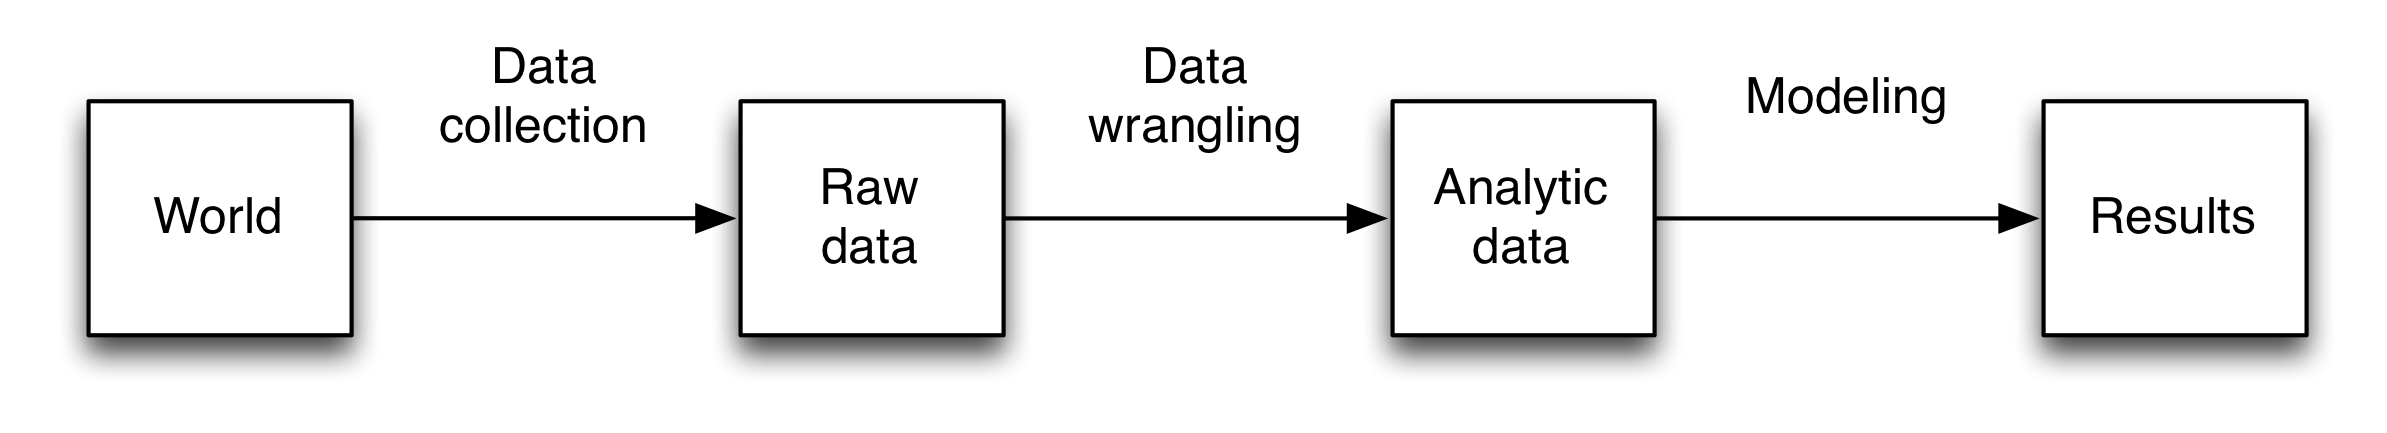
\includegraphics[width=\textwidth]{figures/scientific_pipeline}
\end{center}

\end{frame}
%%%%%%%%%%%%%%%%%%%%%%%%%
\begin{frame}
\frametitle{Building a submission}

Submissions include:
\begin{enumerate}
\item Predictions
\item Code
\item Narrative explanation
\end{enumerate}

\vfill
Submission preparation instructions: \textcolor{blue}{\href{http://www.fragilefamilieschallenge.org/upload-your-contribution/}{www.fragilefamilieschallenge.org/upload-your-contribution/}}

\end{frame}
%%%%%%%%%%%%%%%%%%%%%%%%%%%
\begin{frame}{Get on the leaderboard}

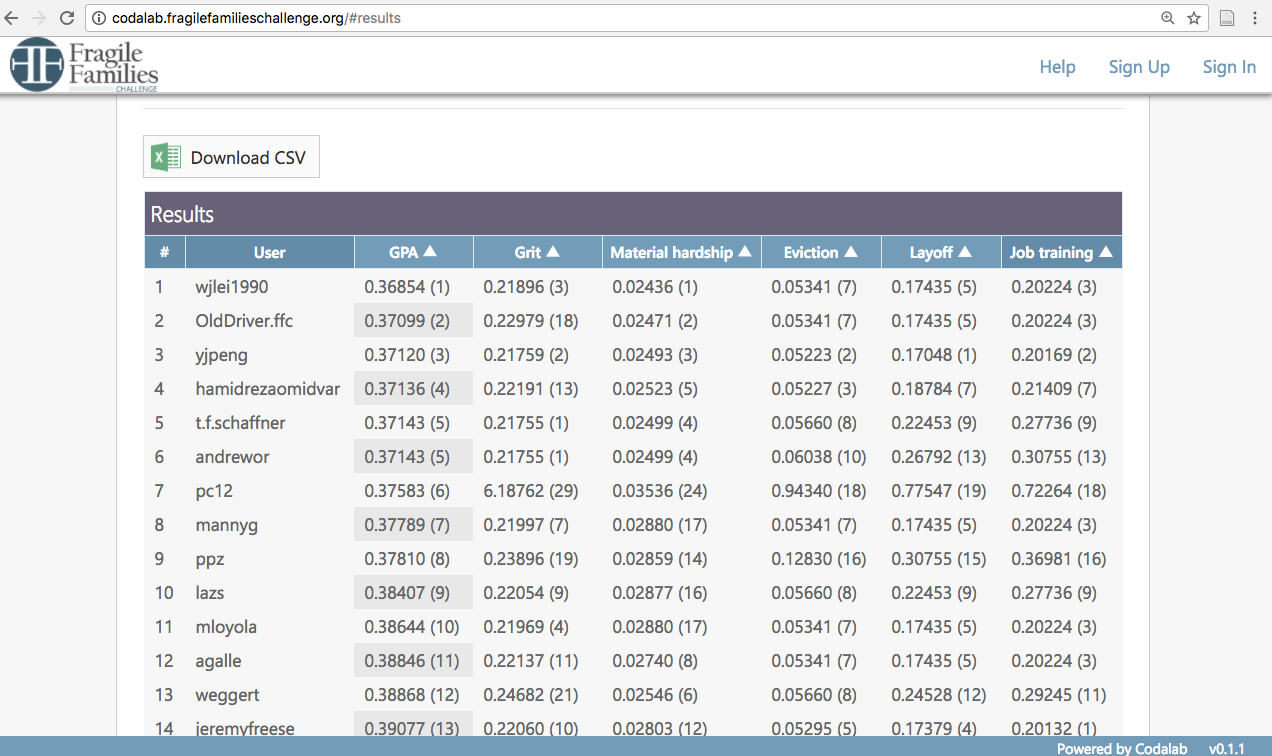
\includegraphics[width = \textwidth]{figures/leaderboard}

\end{frame}
%%%%%%%%%%%%%%%%%%%%%%%%%%%
\begin{frame}

\begin{center}
\LARGE{Advice}
\end{center}

\end{frame}
%%%%%%%%%%%%%%%%%%%%%%%%%%%
\begin{frame}

Most good approaches will likely involve \pause
\begin{itemize}
\item careful data preparation
\pause
\item flexible models that avoid overfitting
\end{itemize}

\end{frame}
%%%%%%%%%%%%%%%%%%%%%%%%%%%
\begin{frame}

\begin{center}
\only<1>{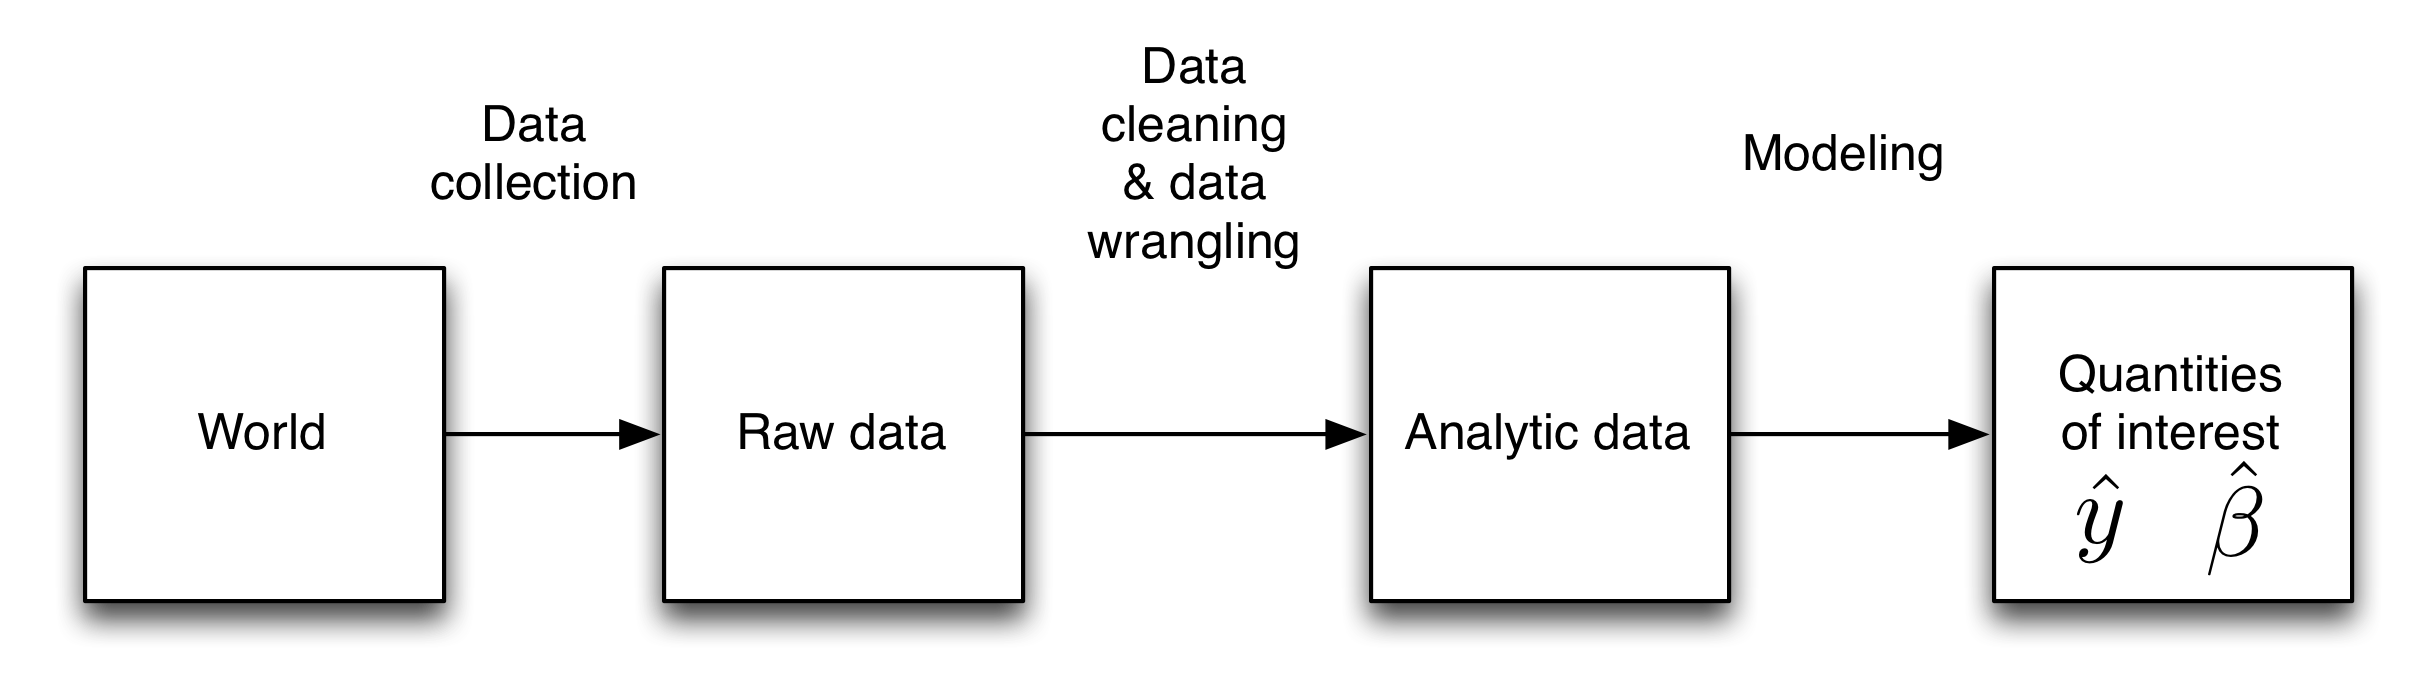
\includegraphics[width=1\textwidth]{figures/data_pipeline}}%
\only<2>{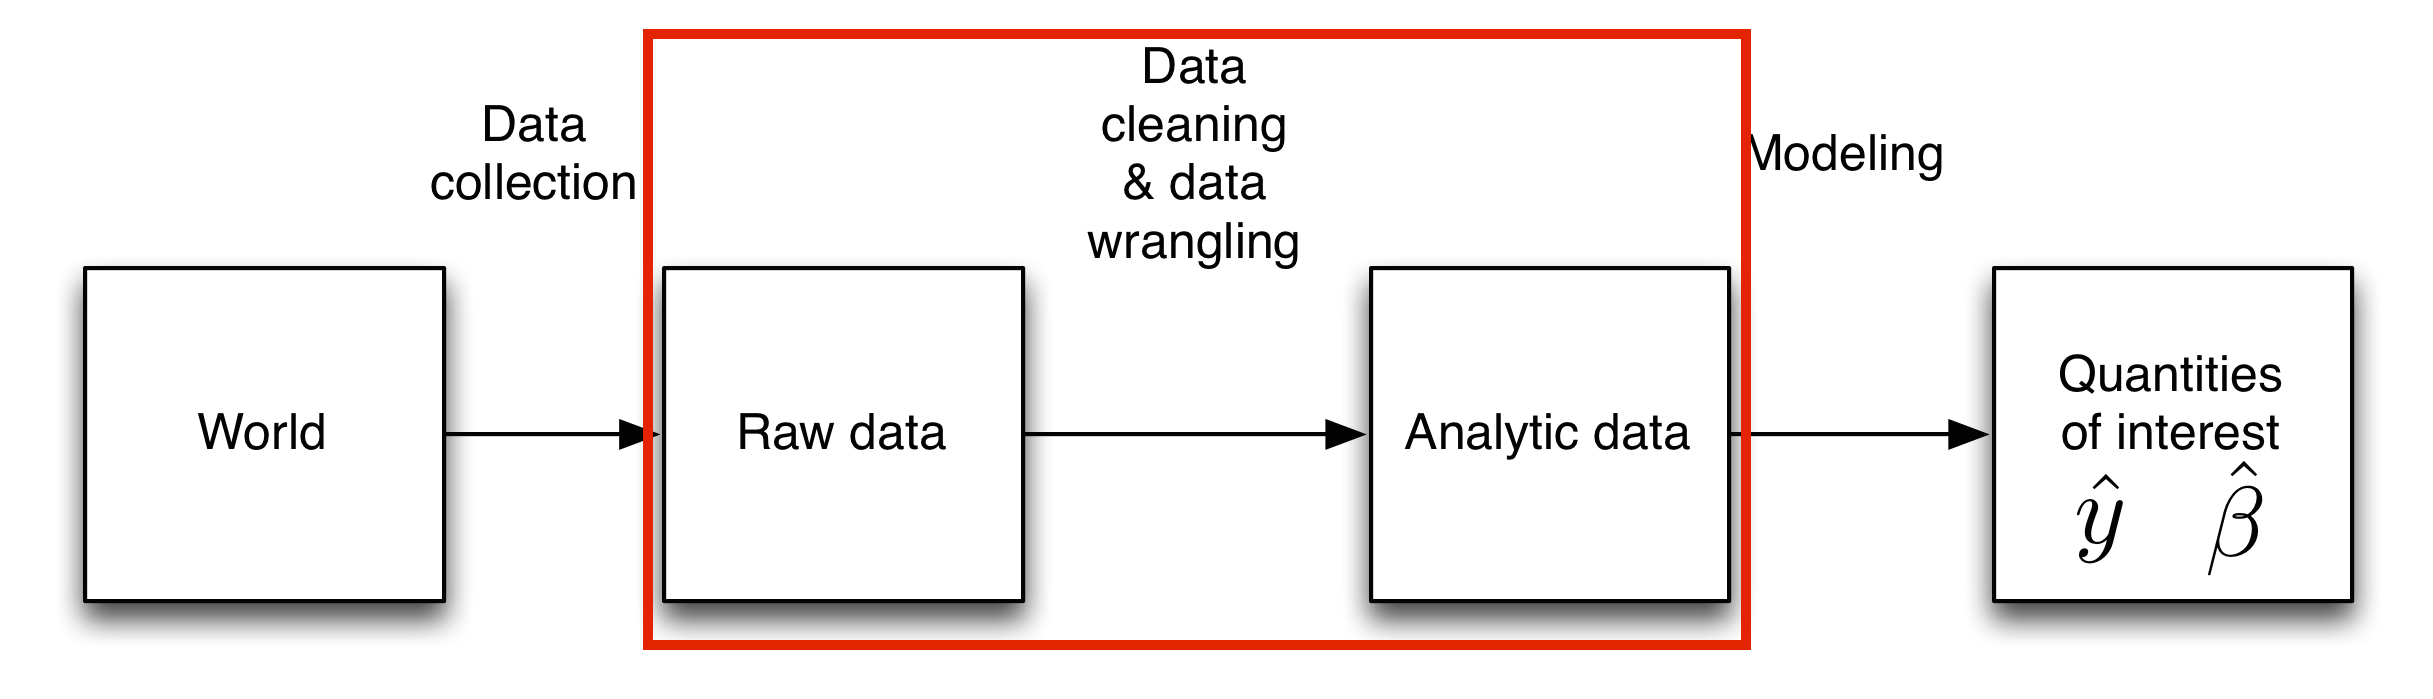
\includegraphics[width=1\textwidth]{figures/data_pipeline_whighlight}}%
\end{center}

\end{frame}
%%%%%%%%%%%%%%%%%%%%%%%%%%%
\begin{frame}

\begin{center}
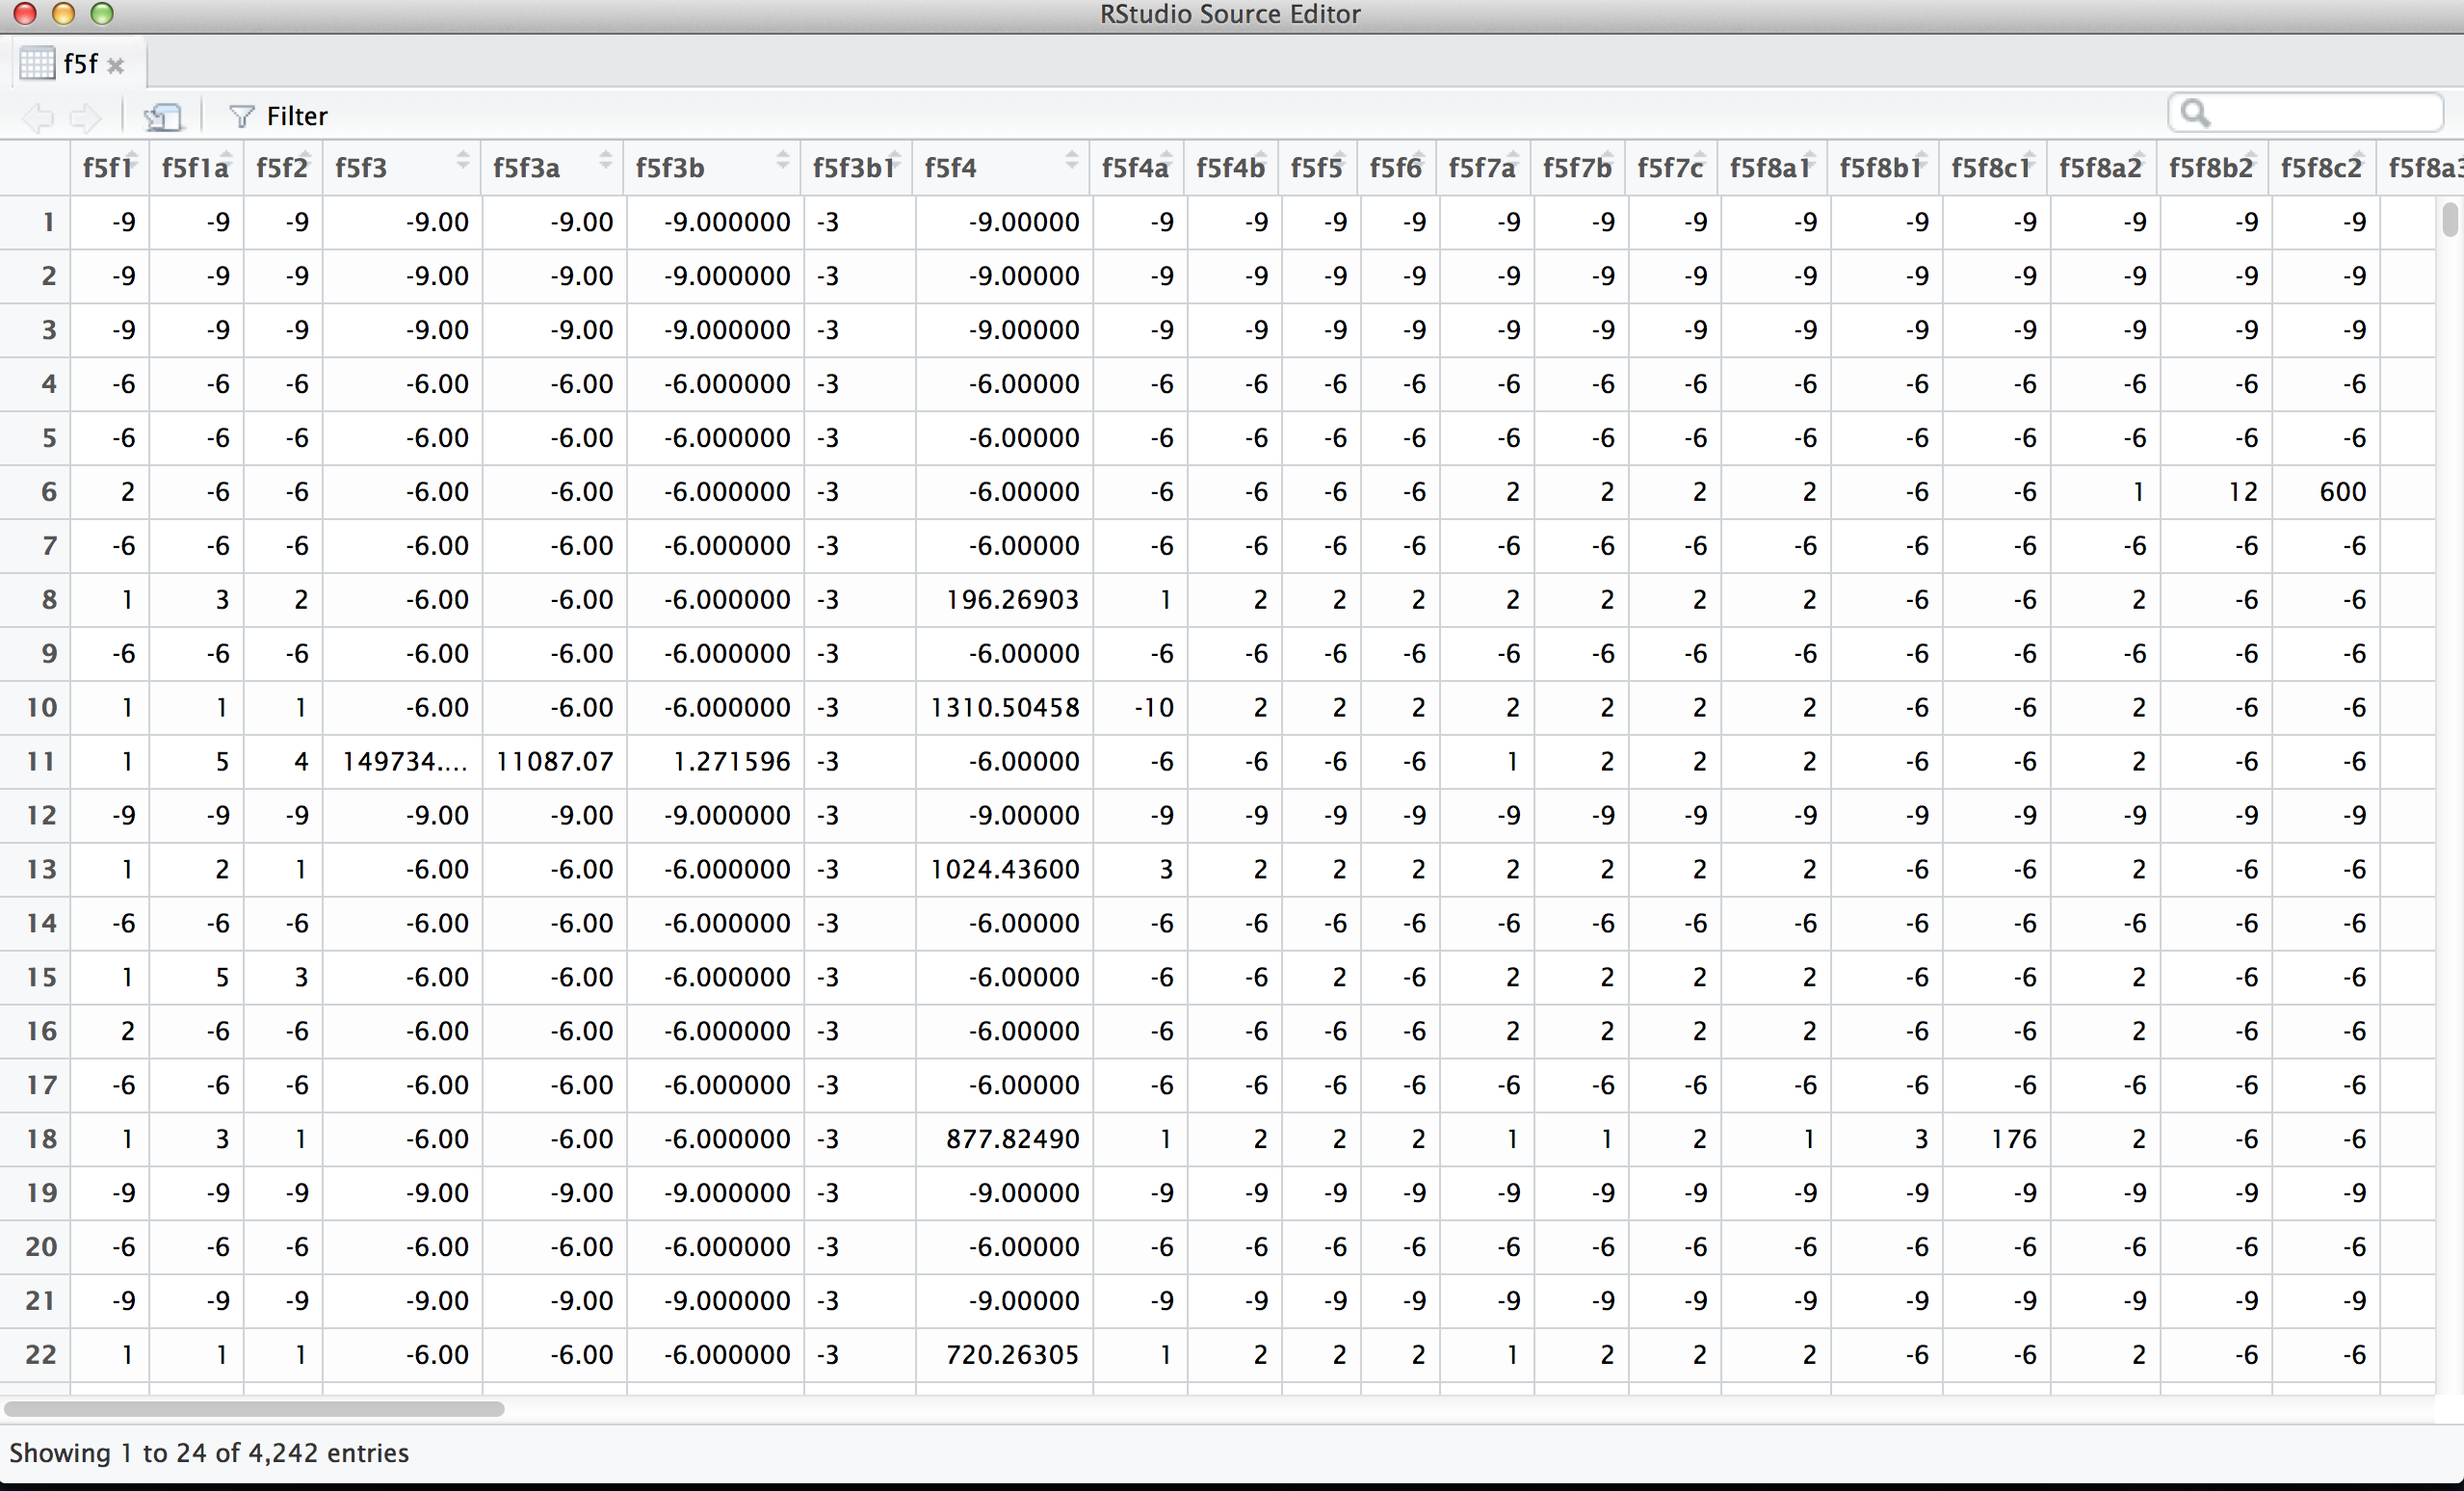
\includegraphics[width=1\textwidth]{figures/ffc_rawdata_f5f}
\end{center}

\end{frame}
%%%%%%%%%%%%%%%%%%%%%%%%%%%
\begin{frame}

\begin{center}
\only<1>{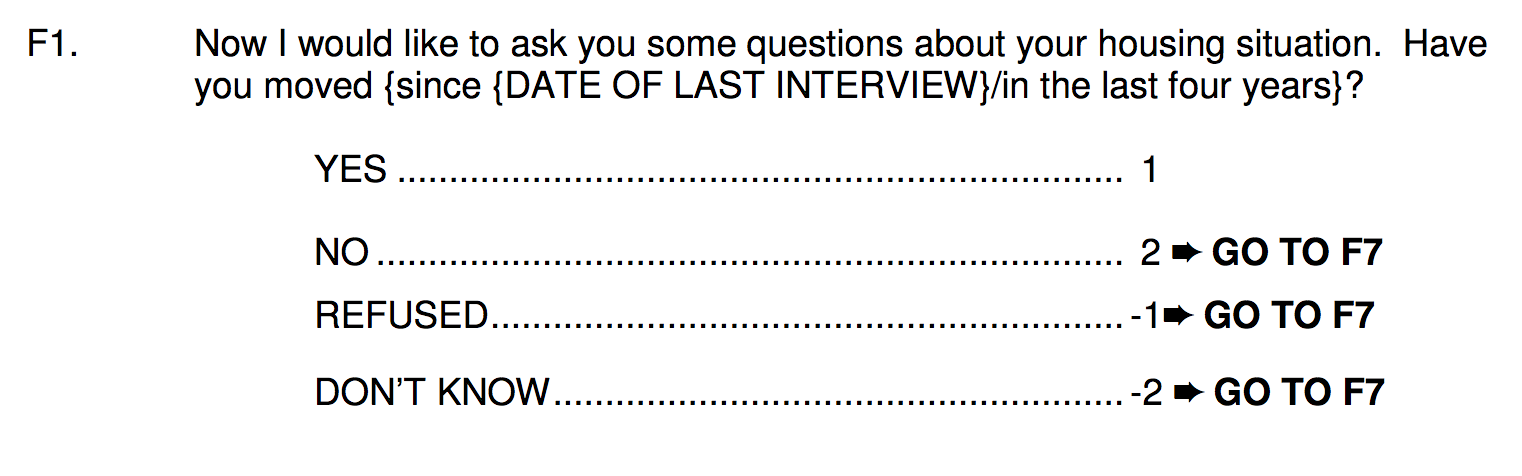
\includegraphics[width=0.95\textwidth]{figures/f5f1}}
\only<2>{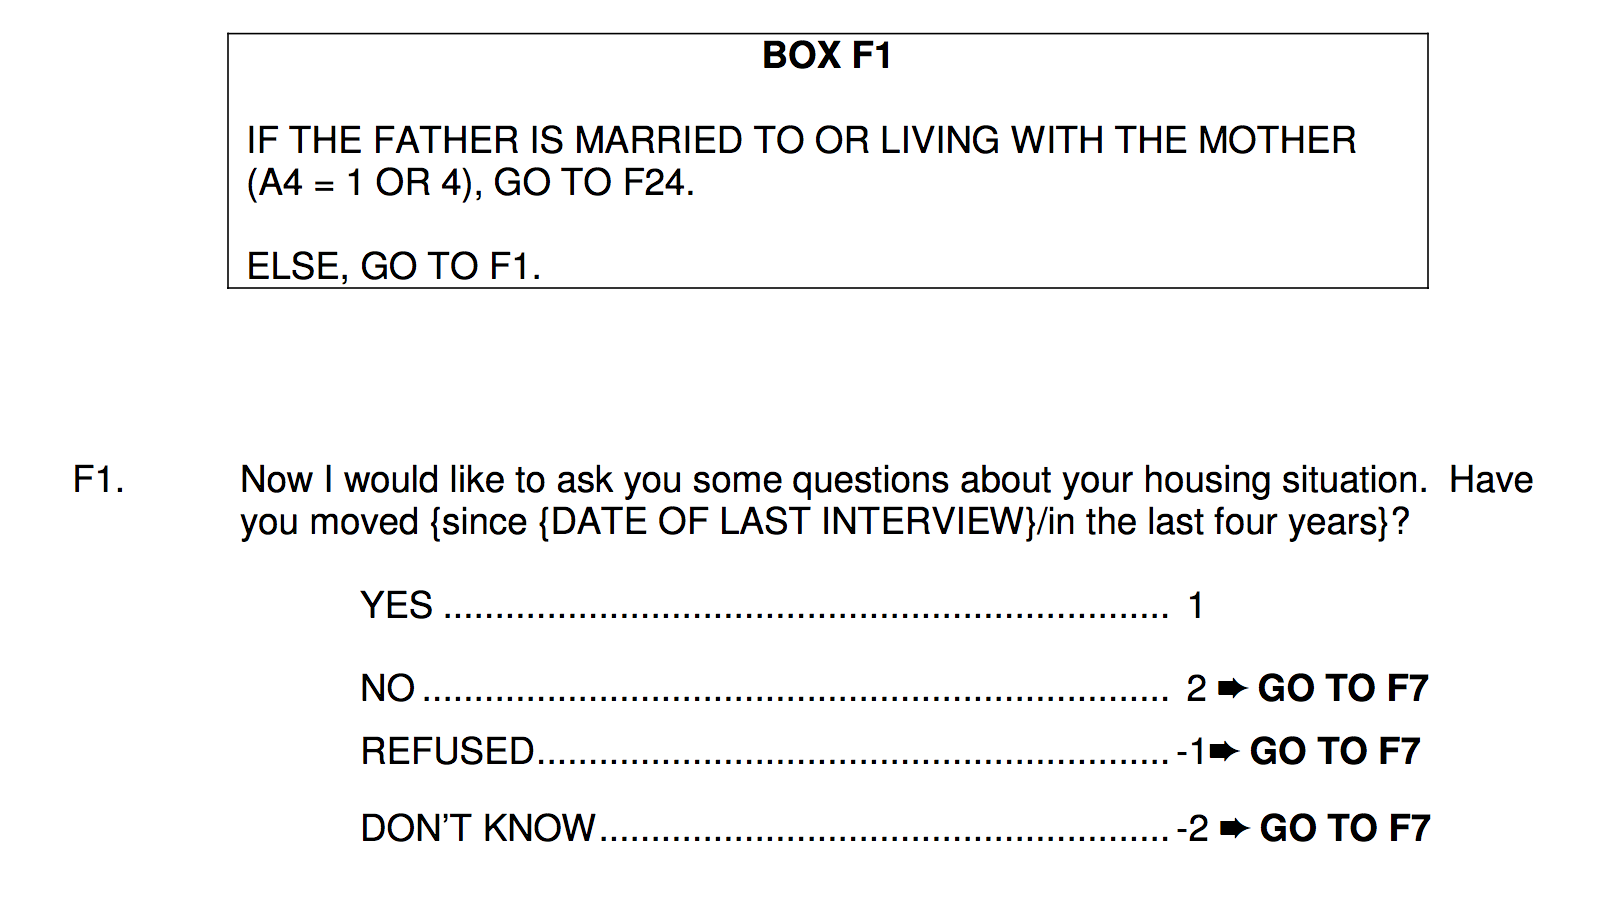
\includegraphics[width=0.95\textwidth]{figures/f5f1_skip}}
\end{center}

\end{frame}
%%%%%%%%%%%%%%%%%%%%%%%%%%%
\begin{frame}

\begin{center}
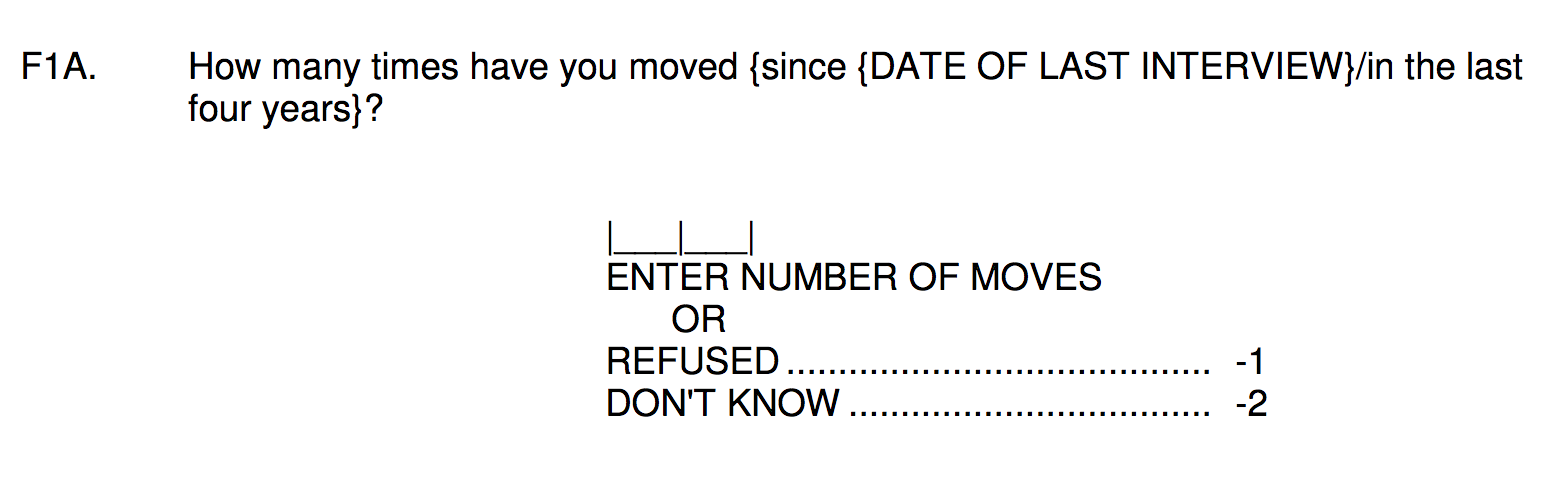
\includegraphics[width=0.95\textwidth]{figures/f5f1a}
\end{center}

\end{frame}
%%%%%%%%%%%%%%%%%%%%%%%%%%%
\begin{frame}

\begin{center}
\only<1>{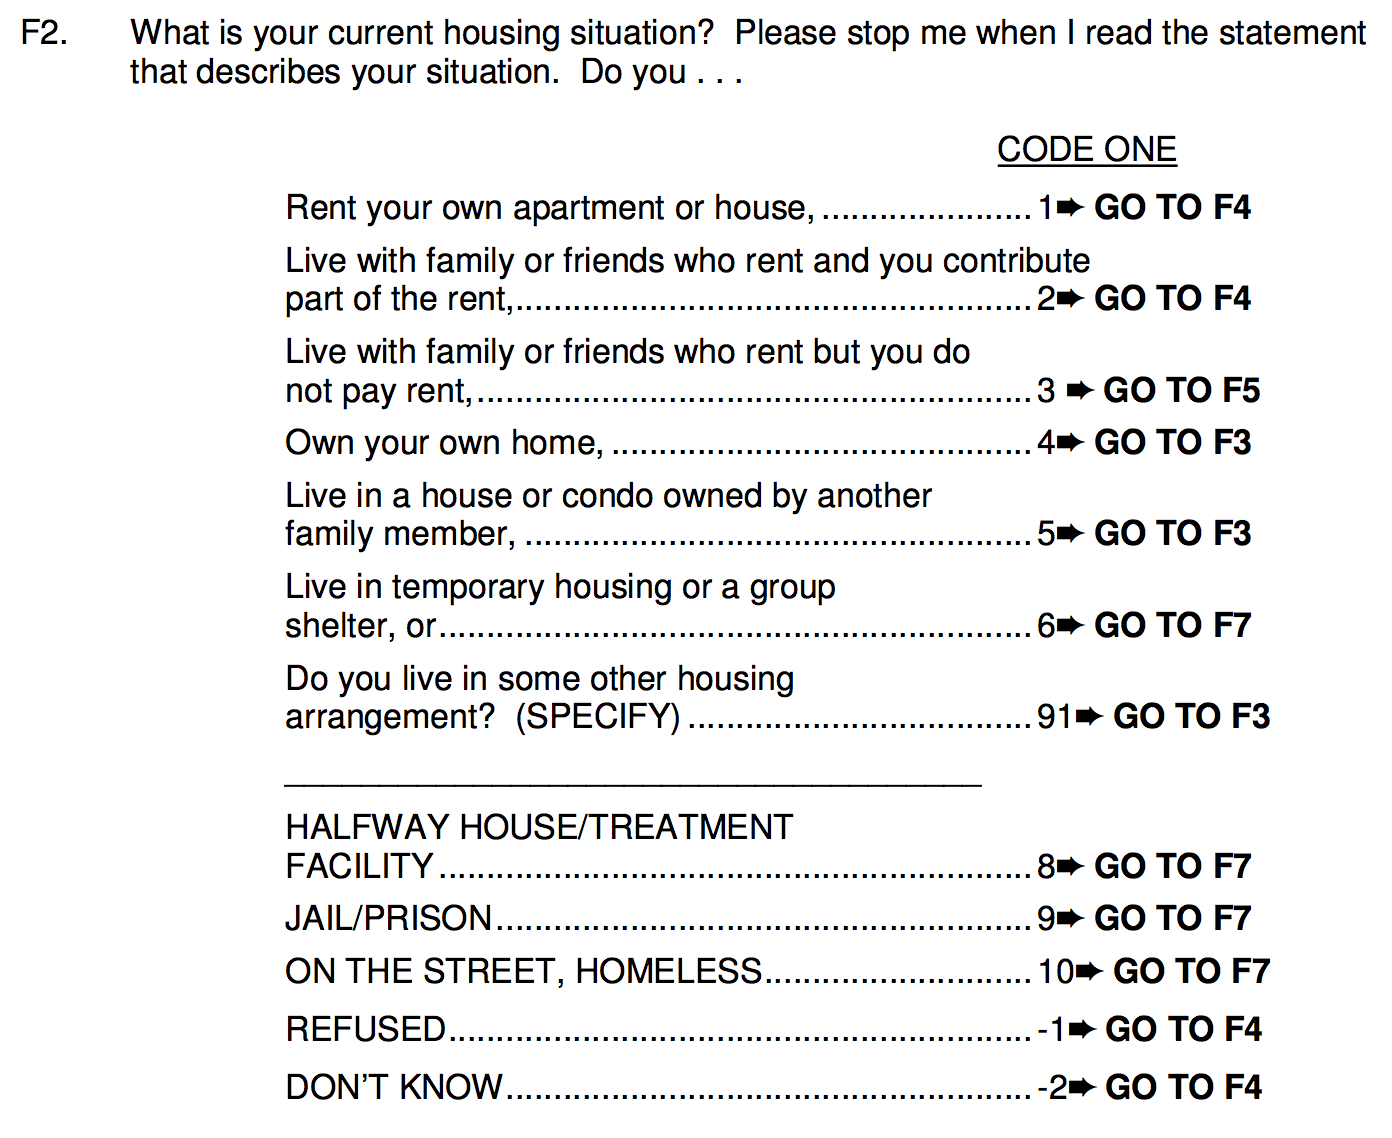
\includegraphics[width=0.95\textwidth]{figures/f5f2}}%
\only<2>{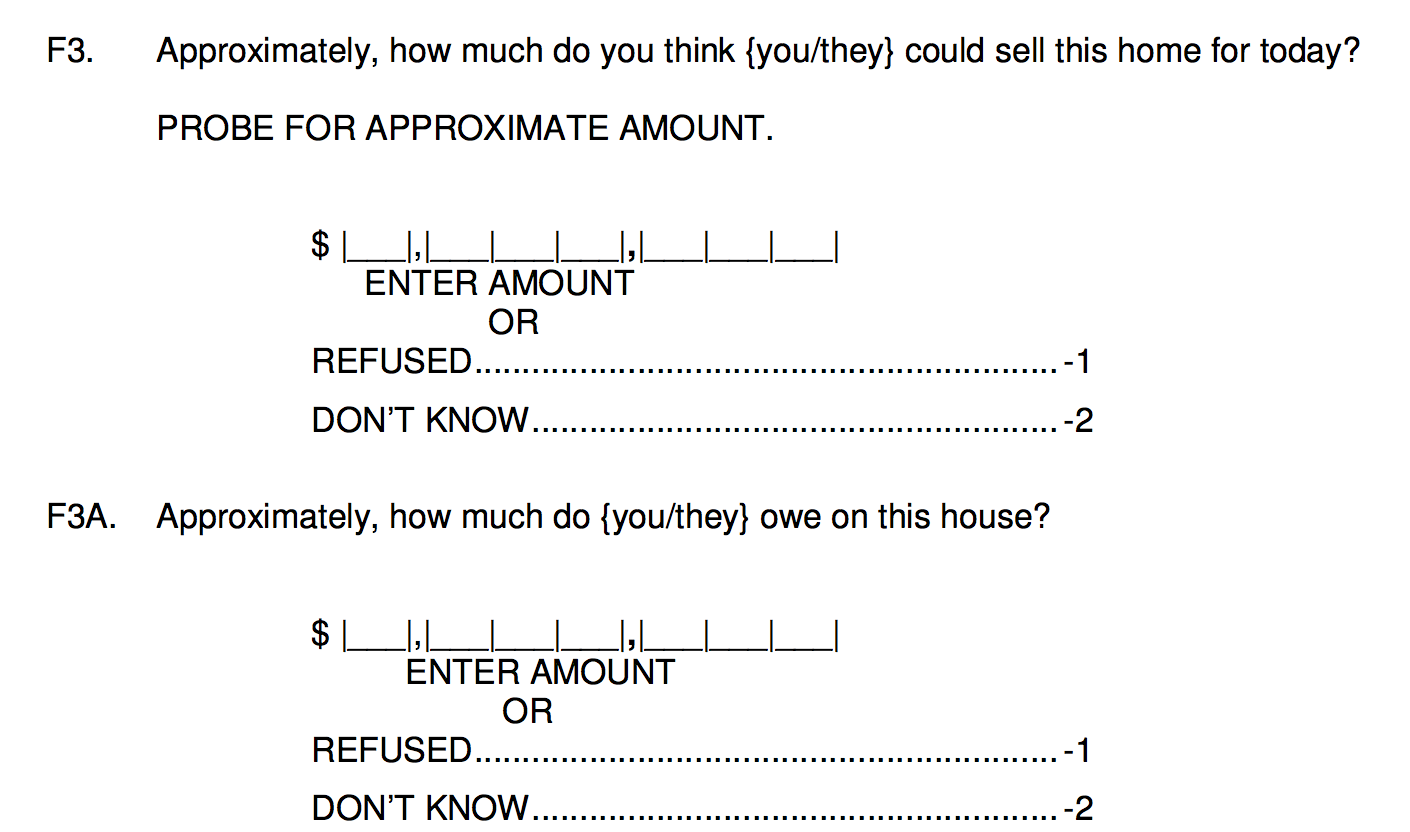
\includegraphics[width=0.95\textwidth]{figures/f5f3_f5f3a}}%
\only<3>{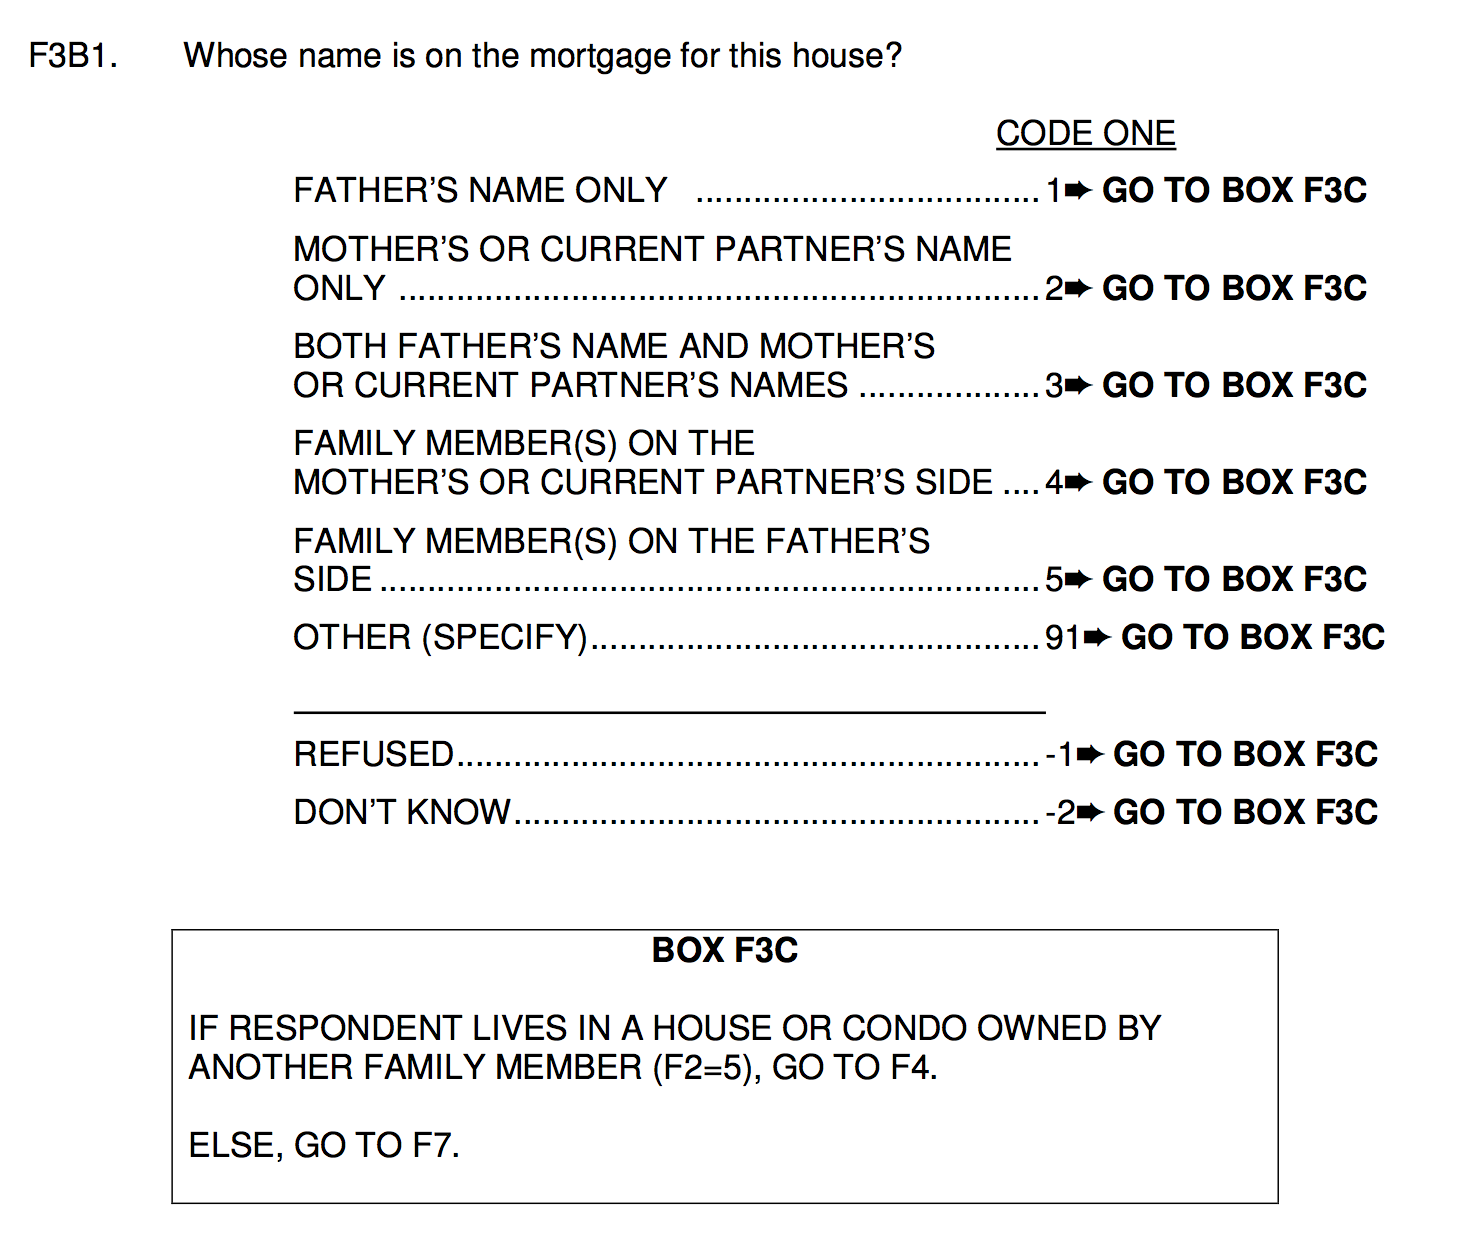
\includegraphics[width=0.95\textwidth]{figures/f5f3b1}}%
\end{center}

\end{frame}
%%%%%%%%%%%%%%%%%%%%%%%%%%%
\begin{frame}

\begin{center}
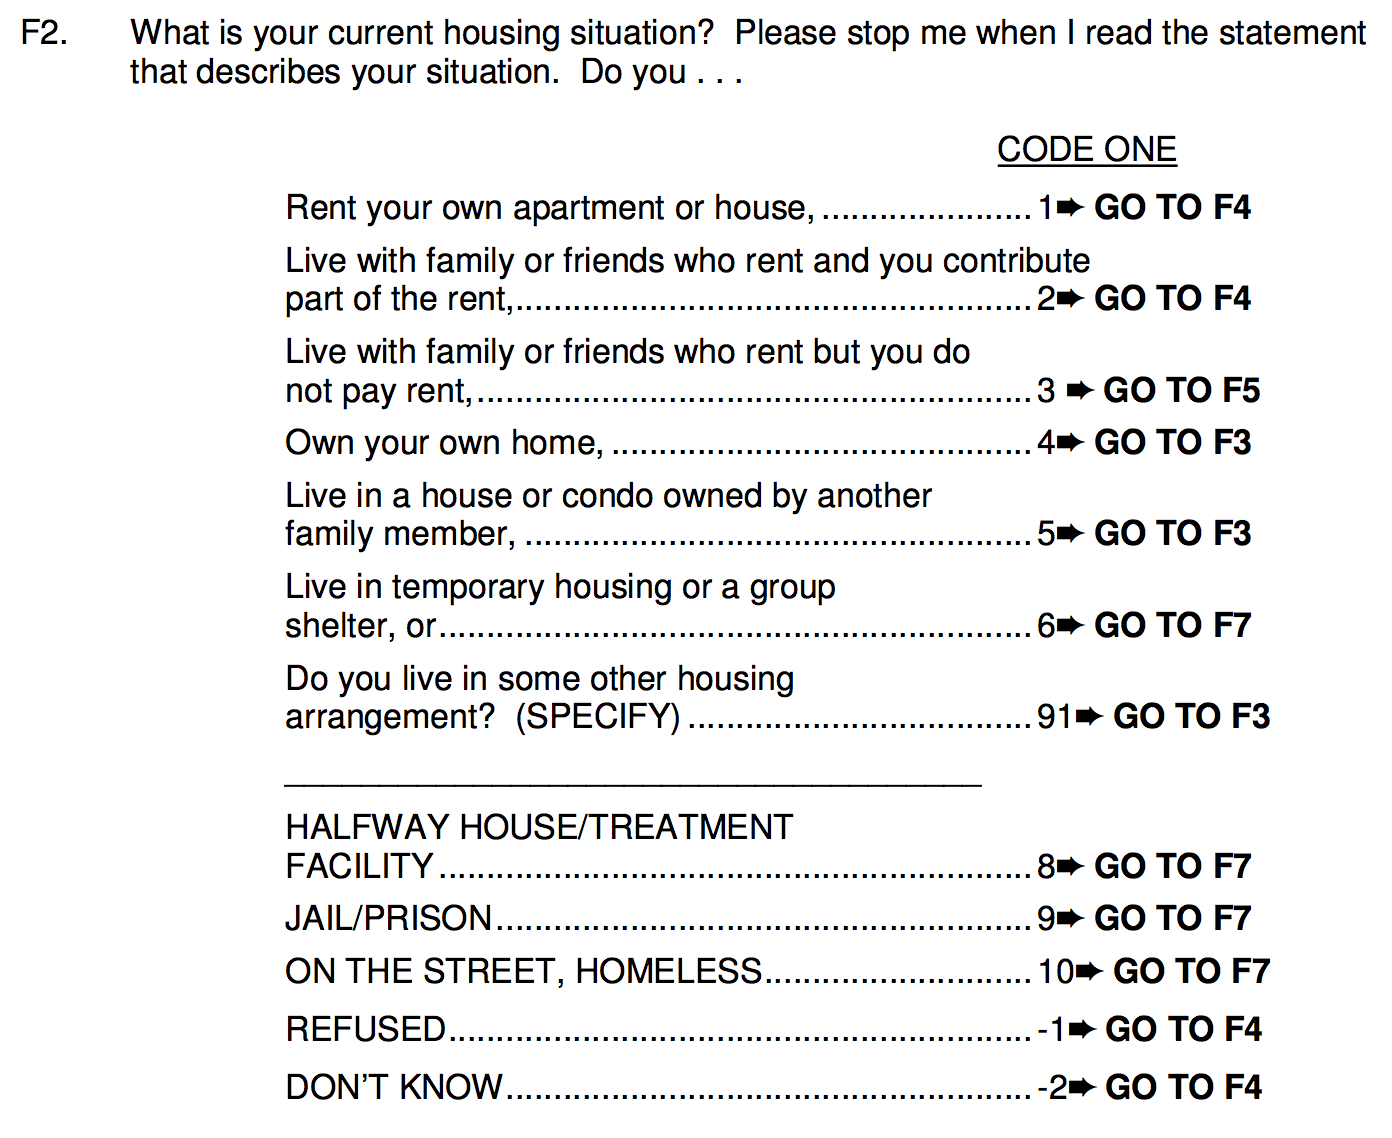
\includegraphics[width=0.95\textwidth]{figures/f5f2}
\end{center}

\end{frame}
%%%%%%%%%%%%%%%%%%%%%%%%%%%
\begin{frame}

This process is \textcolor{blue}{time consuming}.

\begin{center}
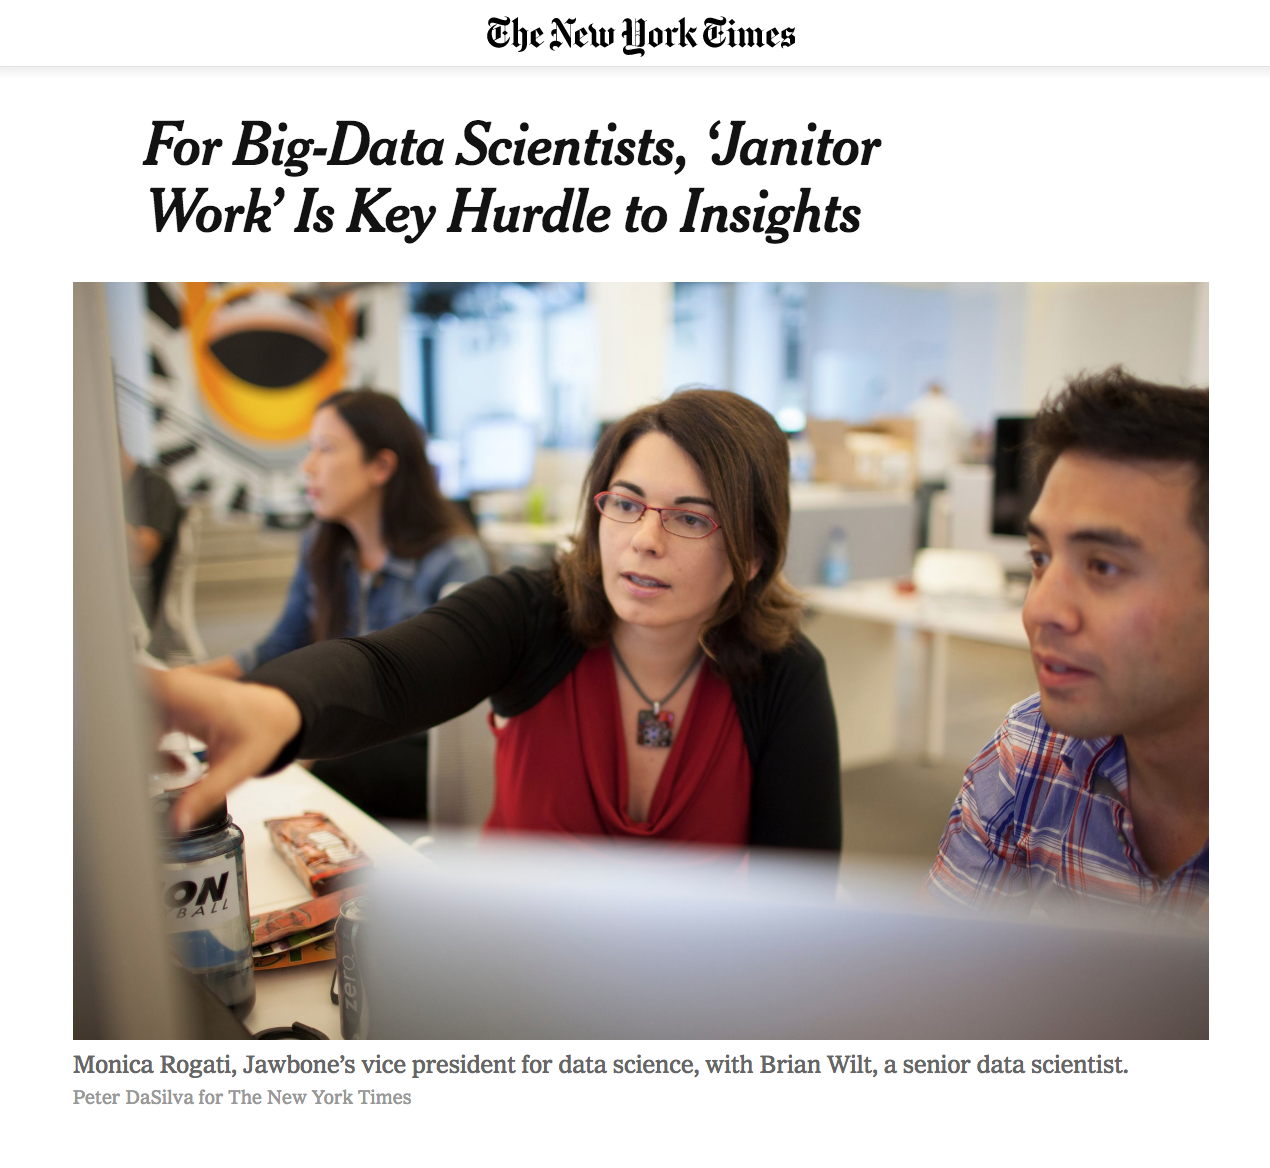
\includegraphics[width=0.65\textwidth]{figures/lohr_for_2014_nytimes_headline}
\end{center}

\vfill
\tiny{\url{https://www.nytimes.com/2014/08/18/technology/for-big-data-scientists-hurdle-to-insights-is-janitor-work.html}}

\end{frame}
%%%%%%%%%%%%%%%%%%%%%%%%%%%
\begin{frame}

This process is \textcolor{blue}{error prone}.

\begin{center}
\only<1>{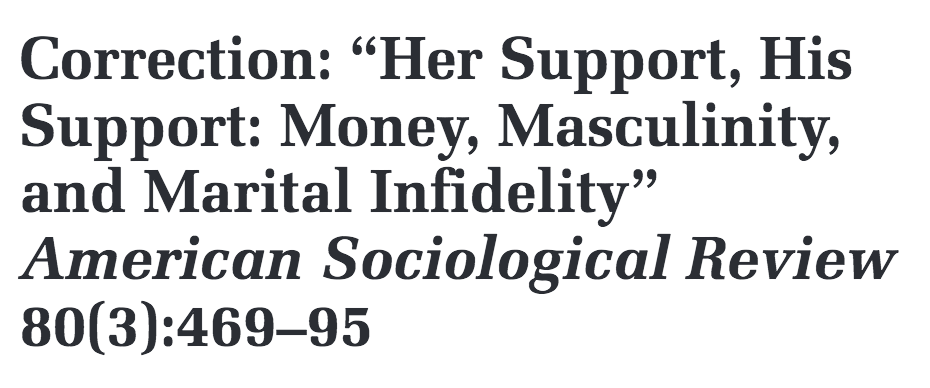
\includegraphics[width=0.95\textwidth]{figures/munsch_correction_2018_title}}%
\only<2>{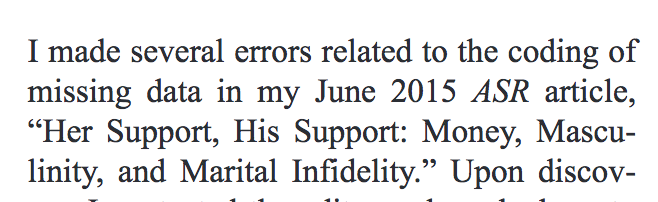
\includegraphics[width=0.95\textwidth]{figures/munsch_correction_2018_firstpara}}%
\end{center}

\end{frame}
%%%%%%%%%%%%%%%%%%%%%%%%%%%
\begin{frame}

This process is \textcolor{blue}{frustrating}.

\begin{center}

\includegraphics[width=0.95\textwidth]{figures/frustrating}
\end{center}

\vfill
\tiny{\url{https://www.talk2solicitors.co.uk/blog/limits-frustration-contract/}}

\end{frame}
%%%%%%%%%%%%%%%%%%%%%%%%%%%
\begin{frame}

Now imagine this \textcolor{blue}{times 100}. \pause We think this data preparation step is a critical barrier to applying machine learning methods to complex survey data.

\begin{center}
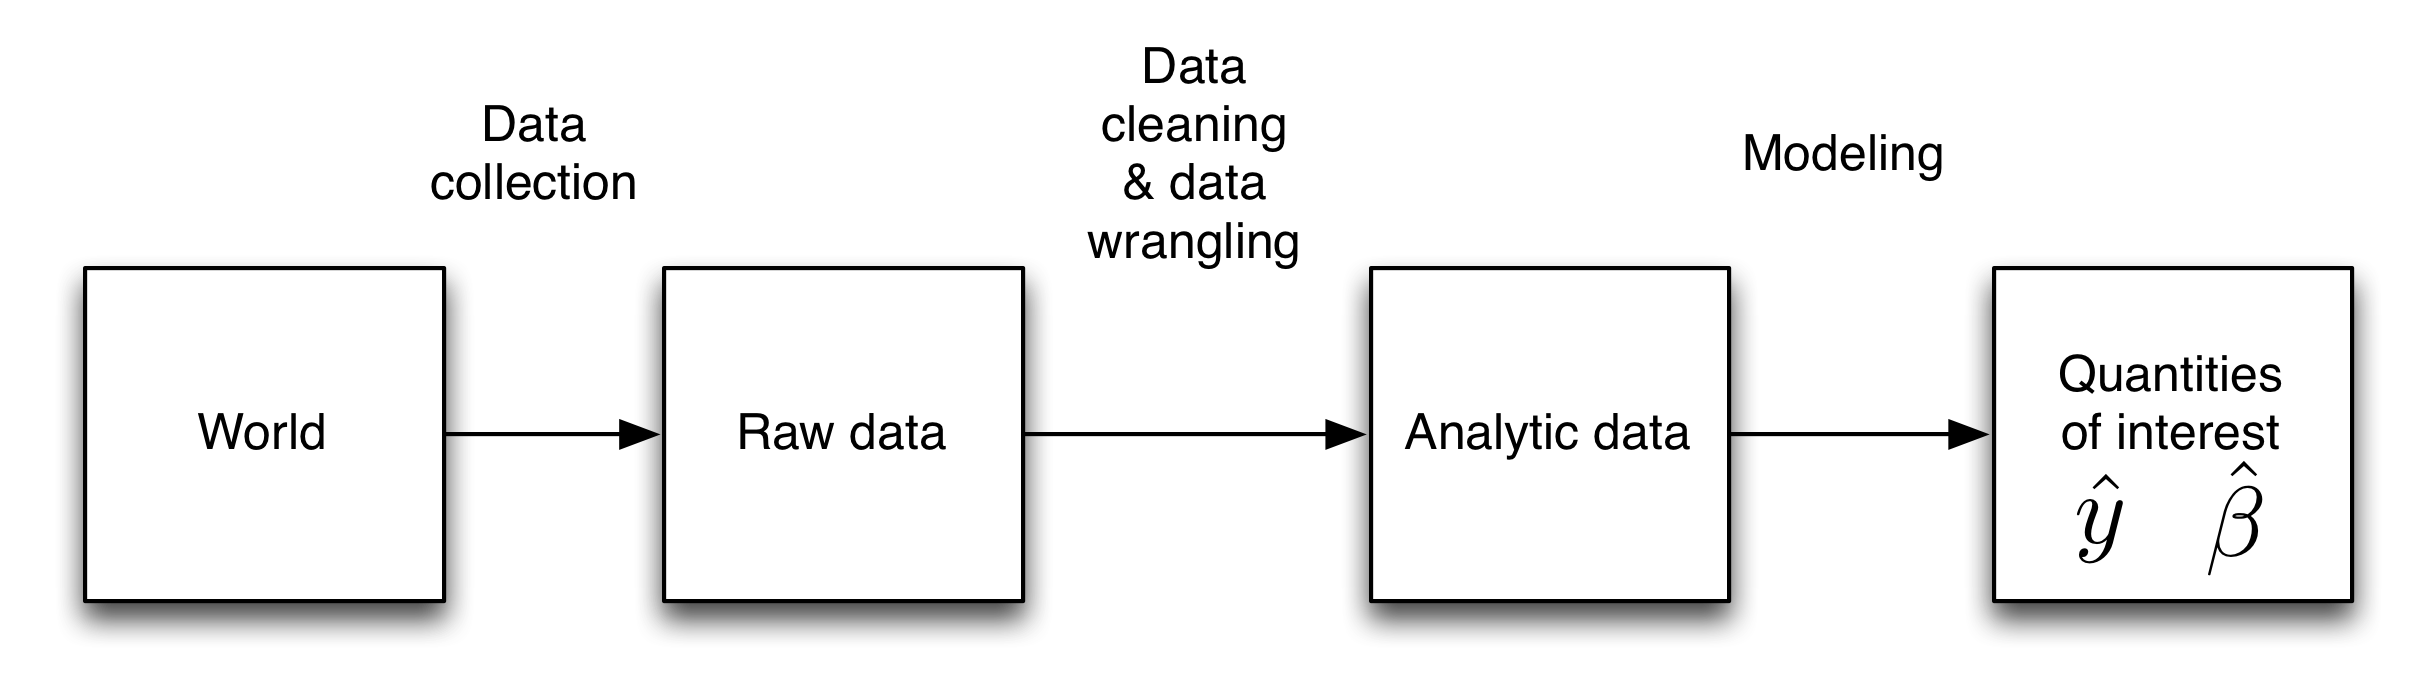
\includegraphics[width=1\textwidth]{figures/data_pipeline}
\end{center}

\end{frame}
%%%%%%%%%%%%%%%%%%%%%%%%%%%
\begin{frame}

\begin{center}
What if this data was as easy to use as your iPhone?
\end{center}

\end{frame}
%%%%%%%%%%%%%%%%%%%%%%%%%%%
\begin{frame}

\begin{center}
\Large{Human-readable $\rightarrow$ machine-actionable}
\end{center}
 
\end{frame}
%%%%%%%%%%%%%%%%%%%%%%%%%%%
\begin{frame}

\begin{itemize}
\item Big team effort: Alexander T. Kindel, Vineet Bansal, Kristin Catena, Tom Hartshorne, Kate Jaeger, Dawn Koffman, Sara McLanahan, Maya Philips, Shiva Rouhani, Ryan Vinh, Matthew J. Salganik \pause
\item Key principle: metadata is data 
\item see Kindel et al (2018) ``\href{https://osf.io/preprints/socarxiv/u8spj/}{Improving metadata infrastructure for complex surveys: Insights from the Fragile Families Challenge}
\end{itemize}

\end{frame}
%%%%%%%%%%%%%%%%%%%%%%%%%%%
\begin{frame}
\frametitle{Data preparation}

\begin{center}
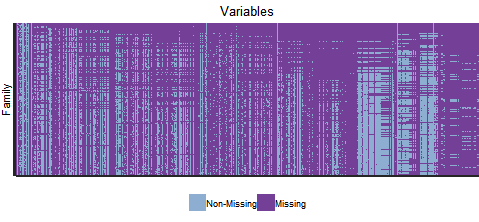
\includegraphics[width = \textwidth]{figures/swissCheese}
\end{center}

\vfill
There are a lot of missing entries in the data matrix

\end{frame}
%%%%%%%%%%%%%%%%%%%%%%%%%%%
\begin{frame}{Common missing codes\footnote{For more complete list and explanation, see \url{http://www.fragilefamilieschallenge.org/missing-data/}\vskip .2cm}}
\frametitle{Data preparation}

Not all missing data is the same
\begin{small}
\begin{itemize}
\item -9 Not in wave - Did not participate in survey/data collection component
\item -6 Valid skip - Intentionally not asked question; question does not apply to respondent or response known based on prior information.
\item -2 Don't know - Respondent asked question; responded ``Don't Know''.
\item -1 Refuse - Respondent asked question; refused to answer question
\item NA also used occasionally
\end{itemize}
\end{small}

\vfill
Given that we have only a few hours, I would recommend not worrying about this.  In the special issue, we saw some evidence that complex approaches to missing data didn't help much.

\end{frame}
%%%%%%%%%%%%%%%%%%%%%%%%%%%
\begin{frame}
\frametitle{Data preparation}

You'll want to deal with unordered categorical variables

\begin{center}
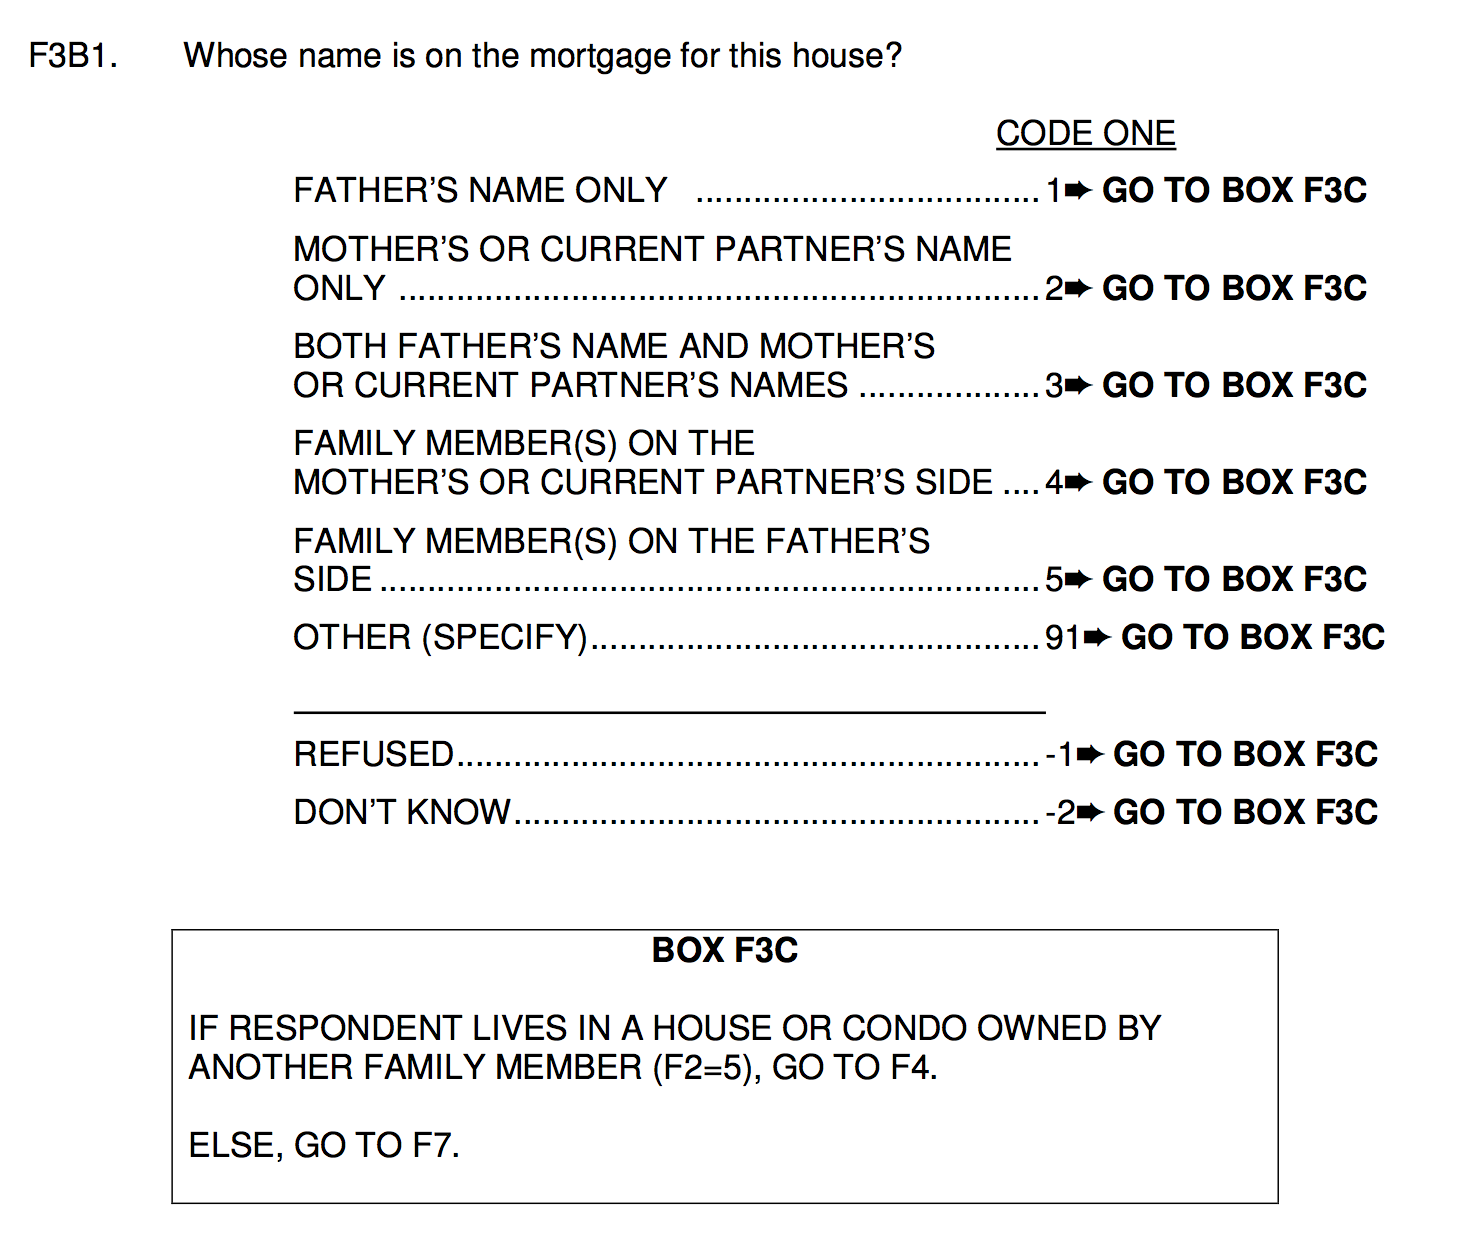
\includegraphics[width=0.95\textwidth]{figures/f5f3b1}
\end{center}

\end{frame}
%%%%%%%%%%%%%%%%%%%%%%%%%%%%
\begin{frame}

What are the main ``recipes'' that people used in the Fragile Families Challenge?
\begin{itemize}
\item data preparation
\item feature selection
\item statistical learning
\end{itemize}

\end{frame}
%%%%%%%%%%%%%%%%%%%%%%%%%%%%
\begin{frame}

Here are the approaches that authors used for data preparation (Key ideas relate to missing data and unordered categorical variables):

\begin{itemize}
\item Mean, median, mode imputation 
\item Missingness indicators
\item Model-based imputation
\item Imputation based on survey structure
\item Constructed variables 
\item Principle component analysis
\item One-hot encoding (dummy variables) 
\item Standardization
\item Transformation
\end{itemize}

\end{frame}
%%%%%%%%%%%%%%%%%%%%%%%%%%%
\begin{frame}

Here are the approaches that authors used for feature selection/variable selection (Key ideas relate to automatic vs manual):

\begin{itemize}
\item Prior expertise
\item Study documentation
\item Literature review
\item F-test
\item Mutual information
\item Dropping low-variance features
\item Multiple datasets
\item Own train/test split
\end{itemize}

\end{frame}
%%%%%%%%%%%%%%%%%%%%%%%%%%%
\begin{frame}
Here are the approaches that authors used for statistical learning (Key ideas are flexibility and over-fitting):

\begin{itemize}
\item general linear model (linear and logistic regression)
\item Tree-based methods (e.g., random forrest, gradient boosted trees)
\item Regularization approaches (e.g., LASSO, Ridge, Elastic Net)
\end{itemize}

\end{frame}
%%%%%%%%%%%%%%%%%%%%%%%%%%%
\begin{frame}

What are the main ``recipes'' that people used in the Fragile Families Challenge?
\begin{itemize}
\item data preparation
\item feature selection
\item statistical learning
\end{itemize}

\end{frame}
%%%%%%%%%%%%%%%%%%%%%%%%%%%%
\begin{frame}
\frametitle{Getting started}

Alex has created \href{https://github.com/compsocialscience/summer-institute/blob/master/2019/materials/day5-mass-collaboration/activity/submission.zip}{a template submission zip file} that includes:
\begin{itemize}
\item predictions.csv (one prediction per family per outcome)
\item narrative (a text file explaining the approach)
\item baseline.R (code to run the submission)
\end{itemize} 

\vfill
You can upload it here:
\large{
\begin{center}
\textcolor{blue}{\href{https://codalab.fragilefamilieschallenge.org/competitions/26}{https://codalab.fragilefamilieschallenge.org/competitions/26}}
\end{center}
}

\end{frame}
%%%%%%%%%%%%%%%%%%%%%%%%%
\begin{frame}

\begin{center}
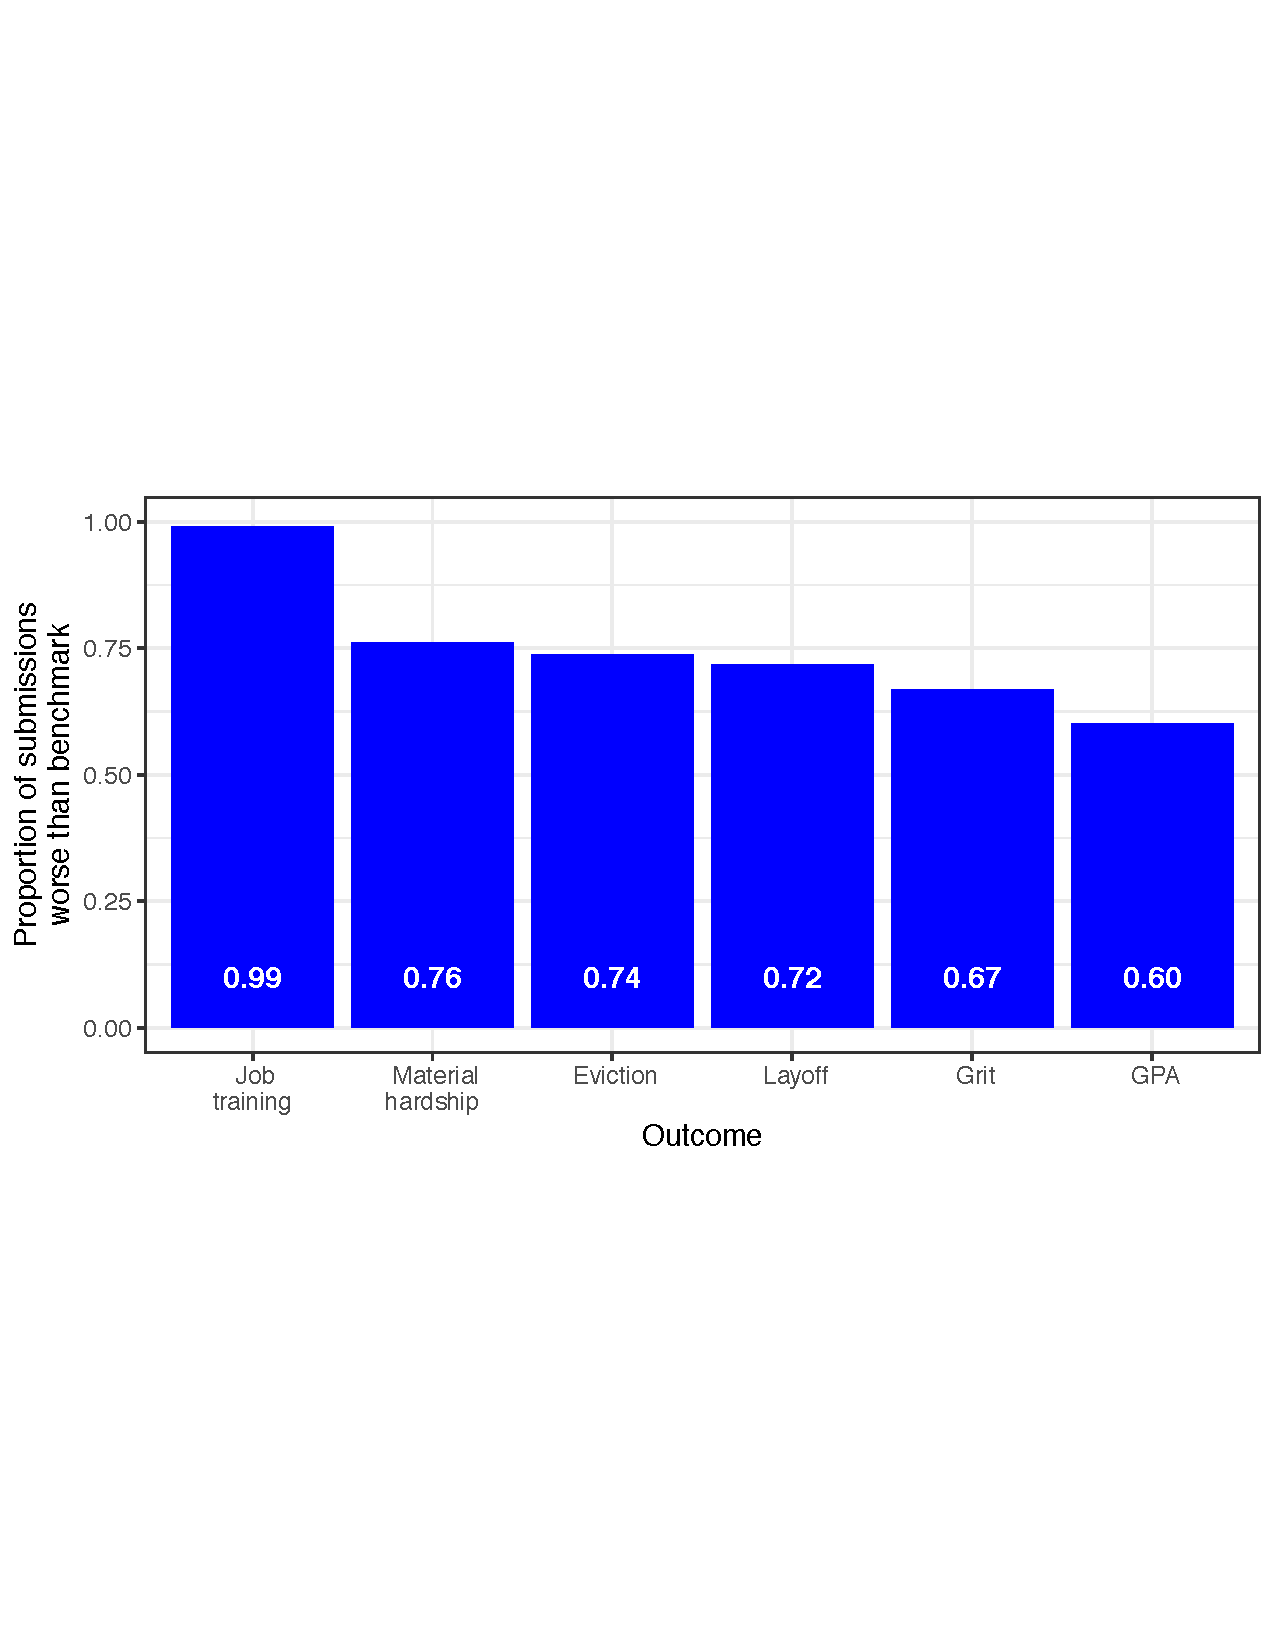
\includegraphics[width=0.95\textwidth]{figures/worse_than_benchmark}
\end{center}

\end{frame}
%%%%%%%%%%%%%%%%%%%%%%%%%
\begin{frame}

\begin{center}
\LARGE Good luck and enjoy
\end{center}

\end{frame}
%%%%%%%%%%%%%%%%%%%%%%%%%%%%%%%%%%%%%%%%%%%%%%%%%%%%%%%%

\end{document}